%!TEX program = xelatex
% 完整编译: xelatex -> bibtex -> xelatex -> xelatex
\documentclass[lang=cn,11pt,a4paper]{elegantpaper}

\usepackage{calc}
\usepackage{times}
\usepackage{float}

\usepackage{titlesec}
\newcommand{\sectionbreak}{\clearpage}

\usepackage{pdfpages}

\usepackage{amssymb} % \Box
%\usepackage{algorithm}  
%\usepackage{algorithmicx}  
\usepackage{algpseudocode}
\usepackage{amsmath}
\usepackage[linesnumbered,ruled,lined]{algorithm2e}
\usepackage{graphicx}
\usepackage{listings}
\usepackage{color}
\usepackage{colortbl}
\usepackage{longtable}
\SetArgSty{textnormal} % non-italics in if-clause of algorithm

\usepackage{hyperref}
\usepackage{titlesec}
\titleformat{\section}{\centering\Huge\bfseries}{\thesection}{1em}{}
\titleformat{\subsection}{\LARGE\bfseries}{\thesubsection}{1em}{}

\title{计算机系统综合实验手册}
% \author{欧先飞 \\ ouxianfei@smail.nju.edu.cn}

%\institute{\href{https://elegantlatex.org/}{Elegant\LaTeX{} 项目组}}

%\newcommand{\blankbox}{\boxed{\textcolor[rgb]{1,1,1}{*}}}
\newcommand{\blankbox}{\Large{\qedsymbol}}

%\version{0.08}
%\date{\zhtoday}

\begin{document}

\maketitle

\tableofcontents

\newpage

\section{基本工具链}

本节所涉及的内容,是为开展计算机系统综合实验的必要基础,请务必完全熟练掌握。

\subsection{git基本用法}

git的教程有很多,这里不详细叙述git的各种基本运作机制,仅从样例出发,讲解必要掌握的命令。

首先是最基本的clone项目:
\begin{lstlisting}
git clone https://github.com/your/repo
git clone git@github.com:your/repo # 需将你的公钥上传到github上
\end{lstlisting}

上传公钥:
\begin{lstlisting}[language=bash]
# 先生成密钥
~bash> cd ~/.ssh && ls -al
. ..
~bash> ssh-keygen -t rsa -C "you@email.cn"
Generating public/private rsa key pair.
Enter file in which to save the key (/home/you/.ssh/id_rsa):
Enter passphrase (empty for no passphrase): 
Enter same passphrase again: 
Your identification has been saved in /home/you/.ssh/id_rsa.
Your public key has been saved in /home/you/.ssh/id_rsa.pub.
The key fingerprint is:
SHA256:ORKaY5n3N4G0P4guAbT0UFNZNorA3mqSL0S0xPWo/+U you@email.cn
The key's randomart image is:
+---[RSA 2048]----+
|..ooo..o+        |
| +=.oo.o .       |
|o+.*..o .        |
| o= o= o +       |
|.o oB o S .      |
|o.+..o + + .     |
|.+ . ...o =      |
|. . o.o  . o     |
| .   o.E         |
+----[SHA256]-----+
~bash> ls # 现在可以看到id_rsa.pub文件
id_rsa  id_rsa.pub
~bash>
\end{lstlisting}
进入github的settings -> SSH and GPG keys -> New SSH Key,然后将id\_rsa.pub的内容拷贝进去即可。

除了克隆项目,还有如下必要用法:
\begin{lstlisting}
git push # 推送
git pull # 拉取
\end{lstlisting}

对远程仓库的管理:
\begin{lstlisting}
git remote -v # 查看远程仓库的情况

# 绑定一个远程仓库git@github.com:new/repo并将其命名为origin
git remote add origin git@github.com:old/repo

# 将仓库名origin所绑定的远程仓库地址更改为git @github.com:new/repo
git remote set-url origin git @github.com:new/repo

# 将本地的local分支推送到远程的remote分支
git push origin local:remote

# 将本地的local分支强制推送到远程的remote分支,如有冲突,覆盖掉远程的项目
git push -f origin local:remote

# 加上-u可以设置缺省推送参数,即后续只需git push即可
git push -u origin local:remote
\end{lstlisting}

对本地项目的管理:
\begin{lstlisting}
# 保存当前目录所有更改并提交到本地仓库
git add . -A && git commit -m 'message'

# 追加提交
git commit --amend -m 'new message'

# 用352cdeca2caa8a309d2所保存的文件覆盖掉当前目录
git checkout 352cdeca2caa8a309d2 .

# 查看352cdeca2caa8a309d2这一提交时README.md的内容
git show 352cdeca2caa8a309d2:./README.md
git show 352cdeca2caa8a309d2:./README.md | vim -

git log # 查看本地项目的变更历史
git reflog # 查看本地项目的完整变更历史,包括所有reset都记录在内
git reset --hard 352cdeca2caa8a309d2 # 回退到352cdeca2caa8a309d2,同时回退目录下的文件
git reset --soft 352cdeca2caa8a309d2 # 只回退git记录,不回退文件内容
\end{lstlisting}

\subsection{makefile}\label{Makefile}

写在前面,对于过于复杂的Makefile,可以使用\lstinline!make -nB target!来查看生成\lstinline!target!时会执行到的指令,这对于了解一个Makefile究竟干了什么非常有用。除此以外Makefile里面可以通过\lstinline!$(info "xxx")!来打印字符串,这个对于调试Makefile非常有用。

\subsubsection{规则依赖}

一个简单的例子:
\begin{lstlisting}
a.o: a.c
  g++ a.c -o a.o

b.o: b.c
  g++ b.c -o b.o

binary: a.o b.o
  echo + binary
\end{lstlisting}

将上述内容写入到你当前目录的Makefile文件中,并保证\lstinline!a.c!和\lstinline!b.c!文件存在,然后在命令行里敲\lstinline!make binary!,这条语句的意思是制造\lstinline!binary!这个目标,make会读特定名称的文件来获取制造这个目标的规则(Makefile是make内置的一个特定名称)。make读取你的Makefile后会发现binary依赖于\lstinline!a.o!和\lstinline!b.o!,并进而计算得出\lstinline!a.o!依赖于\lstinline!a.c!,\lstinline!b.o!依赖于\lstinline!b.c!,最后按照你给定的生成规则\lstinline!g++ a.c -o a.o!和\lstinline!g++ b.c -o b.o!去生成相应的\lstinline!a.o!和\lstinline!b.o!。

敲完\lstinline!make binary!之后,你binary并没有生成,因为你还没有为binary添加生成规则,所以如果你再敲一遍\lstinline!make binary!,相应的\lstinline!echo + binary!语句会被再执行一遍。

我们稍微改一下,让他变成下面这样:
\begin{lstlisting}
a.o: a.c
  g++ a.c -o a.o

b.o: b.c
  g++ b.c -o b.o

binary: a.o b.o
  cat a.o b.o > binary
\end{lstlisting}

这个时候如果你在敲\lstinline!make binary!,生成规则会将\lstinline!a.o!与\lstinline!b.o!拼接成binary文件,由于binary文件是最新生成的,它的时间戳大于\lstinline!a.o!和\lstinline!b.o!的时间戳,所以再下一次你敲\lstinline!make binary!的时候,make会输出\lstinline!'binary' is up to date!。

一般而言,我们并不希望我们所生成的中间文件和源码文件共用一个目录,假设我们希望将目录结构调整成这样:
\begin{lstlisting}
+---src
|   +--- a.c
|   +--- b.c
|
+---build
    +--- a.o
    +--- b.o
    +--- binary
\end{lstlisting}

为了达成这个目的,我们需要对Makefile做一些微调:
\begin{lstlisting}
build/a.o: src/a.c
  mkdir -p build
  g++ src/a.c -o build/a.o

build/b.o: b.c
  mkdir -p build
  g++ src/b.c -o build/b.o

build/binary: build/a.o build/b.o
  cat build/a.o build/b.o > build/binary
\end{lstlisting}

相应的,基于这个Makefile来生成binary,我们需要执行\lstinline!make build/binary!,这条命令会按照你的规则去生成\lstinline!build/a.o!和\lstinline!build/b.o!两个文件,然后拼接成\lstinline!build/binary!这个文件。

这个时候,你可能发现,make的时候连目录一起写进去太撒刁了,所以这个Makefile可以进一步改进:

\begin{lstlisting}
.PHONY: binary

binary: build/binary

build/a.o: src/a.c
  mkdir -p build
  g++ src/a.c -o build/a.o

build/b.o: b.c
  mkdir -p build
  g++ src/b.c -o build/b.o

build/binary: build/a.o build/b.o
  cat build/a.o build/b.o > build/binary
\end{lstlisting}

\lstinline!.PHONY!的作用是定义一个伪目标,什么是伪目标,直观的讲就是,这个目标在磁盘上不存在。之前Makefile里面的\lstinline!a.o!、\lstinline!build/binary!、\lstinline!build/a.o!这些目标在磁盘上是会对应到一个实际存在的文件的,而伪目标不需要满足这个要求,同时相应的,make也不会去检查伪目标的时间戳,而是直接调用他的生成规则,比如:

\begin{lstlisting}

.PHONY: hello

hello:
  touch hello
  echo hello world
\end{lstlisting}

在这个makefile中,无论你敲几次\lstinline!make hello!,\lstinline!touch hello!和\lstinline!echo hello world!这两条生成规则都会被执行。

\subsubsection{通用匹配\%和生成规则简化}

在上文提到的Makefile中,你会发现在编写a.o和b.o的生成规则的时候,你需要把\lstinline!build/!和\lstinline!a.o!这样的多余的东西再写一遍,这个信息明明已经包含在依赖目标和生成目标里了,为了简化规则的编写,makefile定义了一系列的简写符号,用这些符号我们可以将Makefile简化成:

\begin{lstlisting}
.PHONY: binary

binary: build/binary

build/a.o: src/a.c
  mkdir -p $(@D)
  g++ $^ -o $@

build/b.o: b.c
  mkdir -p $(@D)
  g++ $^ -o $@

build/binary: build/a.o build/b.o
  cat $^ > $@
\end{lstlisting}

其中\lstinline!$^!出现在生成规则中表示所有被依赖的目标(示例中\lstinline!$^!会被替换成\lstinline!build/a.o build/b.o!),\lstinline!$@!表示生成的目标(示例中上下两条生成规则里的\lstinline!$@!分别会被替换成\lstinline!build/a.o!和\lstinline!build/b.o!),\lstinline!$(@D)!则是表示生成目标所在的目录,也就是\lstinline!build/!,所以上面的Makefile其实与之前的Makefile完全等价。

\begin{table}[htbp]
\centering
\begin{tabular}{|c|c|}
\hline
符号&含义 \\\hline
\lstinline|$(@D)| & 当前规则目标所在目录 \\\hline
\lstinline|$@| & 当前规则目标 \\\hline
\lstinline|$<| & 当前规则依赖项的第一个 \\\hline
\lstinline|$^| & 当前规则的所有依赖项 \\\hline
\end{tabular}
\caption{规则匹配中常见符号}
\end{table}

到这里,你会发现一件更撒刁的事,那就是\lstinline!mkdir -p $(@D)!和\lstinline!g++ $^ -o $@!这两条语句你在两个目标的生成规则中写了两遍,为了解决这样的问题,Makefile又提供了通配符机制,利用通配符,我们可以将Makefile进一步改写成:

\begin{lstlisting}
.PHONY: binary

binary: build/binary

build/%.o: src/%.c
  mkdir -p $(@D)
  g++ $^ -o $@

build/binary: build/a.o build/b.o
  cat $^ > $@
\end{lstlisting}

在这个Makefile上,如果我们敲\lstinline!make binary!,make会去查找\lstinline!build/binary!所依赖的\lstinline!build/a.o!和\lstinline!build/b.o!的生成规则,当然make是找不到的,因为我们并没有明确的写这样的规则。但是make会进一步发现,它只要把\lstinline!build/%.o!中的\lstinline!%!这个字符替换成\lstinline!a!,他就能匹配上\lstinline!build/%.o: src/%.c!这条规则,于是它就把这条规则里面所有的\lstinline!%!都替换成了\lstinline!a!,便得到了\lstinline!build/a.o!的生成规则,同理它也能获得\lstinline!build/b.o!的生成规则。

\subsubsection{变量和函数的使用}

在上面的Makefile里面,我们还有着这样一个问题,就是如果我们不知道src下面究竟有多少\lstinline!.c!文件,但是我们依旧希望Makefile能工作应该怎么办。举个简单的场景,你的项目正在如火如荼的发展中,每天都可能添加若干个\lstinline!.c!文件或重命名若干个\lstinline!.c!文件,如果你每次都要手动更新Makefile,未免太过撒刁了,为了解决这个问题,Makefile提供了函数机制。

回顾我们的需求,我们其实需要的是make能自动找到src下所有的.c文件,并将其重命名为build下的.o文件,最后放到\lstinline!build/binary!的依赖目标中去:

\begin{lstlisting}
.PHONY: binary

binary: build/binary

build/%.o: src/%.c
  mkdir -p $(@D)
  g++ $^ -o $@

build/binary: $(patsubst src/%.c,build/%.o,$(shell find src/ -name "*.c"))
  cat $^ > $@
\end{lstlisting}

新的Makefile中\lstinline!build/binary!所依赖的目标已经被替换成了\lstinline!$(patsubst src/%.c,build/%.o,$(shell find src/ -name "\*.c"))!,我们分开来讲这条语句,首先是\lstinline!$(shell find src/ -name "\*.c")!,这条语句会调用你终端中的\lstinline!find!命令,查找\lstinline!src!目录下所有的\lstinline!.c!文件,并将其替换成查找的结果,也就是说这条语句执行完毕之后原语句会变成\lstinline!$(patsubst src/%.c,build/%.o,src/a.c src/b.c)!,\lstinline!patsubst!是make的一个内置函数,它的作用是根据你指定的初始特征和结果特征,对你的输入进入转化,对应到这条语句,你给它的初始特征是\lstinline!src/%.c!,结果特征是\lstinline!build/%.o!,输入是\lstinline!src/a.c src/b.c!,对于输入中的每一项,如\lstinline!src/a.c!,\lstinline!patsubst!函数会发现将\lstinline!%!换成\lstinline!a!就能匹配上,然后他讲结果特征中的\lstinline!%!也换成\lstinline!a!,并将结果替换掉\lstinline!src/a.c!,也就是说,\lstinline!src/a.c!会被替换成\lstinline!build/a.o!,同理\lstinline!src/b.c!也会被替换成\lstinline!build/b.o!。

上述Makefile看着非常蛋疼,因为我们写了一个超长的语句,有没有一种机制,像编程语言一样,通过定义一些中间变量来拆分超长表达式呢?答案当然是有的,所以上面的Makefile又可以改成下面这样:

\begin{lstlisting}
.PHONY: binary

SRC_DIR := src/
SRCS    := $(shell find $(SRC_DIR) -name "*.o")
OBJ_DIR := build/
OBJS    := $(patsubst src/%.c,build/%.o,$(SRCS))

binary: $(OBJ_DIR)binary

$(OBJ_DIR)%.o: $(SRC_DIR)%.c
  mkdir -p $(@D)
  g++ $^ -o $@

$(OBJ_DIR)binary: $(OBJS)
  cat $^ > $@
\end{lstlisting}

上面的赋值使用了\lstinline!:=!,你暂时不需要知道为什么是\lstinline!:=!而不是\lstinline!=!,如果你真的想了解,在docs目录下的Makefile.pdf可以给你答案,同时如果哪天你需要什么其它的功能,你也可以通过查阅\lstinline!Makefile.pdf!来看看是否有相应的函数。

\begin{table}[htbp]
\centering
\begin{tabular}{|c|c|}
\hline
函数&含义(具体用法请查询\href{run:../manuals/Makefile.pdf}{手册}) \\\hline
\lstinline|$(shell xxx)| & 执行shell命令,并将结果替换到当前位置 \\\hline
\lstinline|$(dir ...)| & 获取目录 \\\hline
\lstinline|$(notdir ...)| & 获取文件名 \\\hline
\lstinline|$(realpath ...)| & 将相对路径转化为绝对路径 \\\hline
\lstinline|$(abspath ...)| & 将相对路径转化为绝对路径 \\\hline
\lstinline|$(foreach v, ..., ...)| & 遍历 \\\hline
\lstinline|$(eval ...)| & 根据输入的字符串生成新规则 \\\hline
\lstinline|$(subst , , ...)| & 子串替换 \\\hline
\lstinline|$(patsubst , ..., ...)| & 基于特征的子串替换 \\\hline
\end{tabular}
\caption{Makefile常用函数}
\end{table}

\subsubsection{宏的使用与自动规则生成}

假如你想把你的Makefile包装成一个功能库,其他人只要include你的Makefile就能获得上述所有的功能,那么你需要怎么做呢?一个简单的答案就是宏。

待续。。。

\subsection{verilator}\label{verilator}
verilator可以将我们的verilog代码使用C++模拟,从而使用C++语言可以编写测试程序。verilator将我们的verilog代码编译成一个类,我们只需要在我们的测试的.c文件中include其生成的头文件即可。

\subsubsection{前置说明}
verilator的用法,在样例工程中均有体现,建议从样例工程入手,辅之以手册博客,样例项目参见\href{run:../examples/1.Makefile-chisel-sample}{examples/1.Makefile-chisel-sample}。

\subsubsection{使用makefile组织verilator}
从样例项目出发,组织一个工程的makefile,首先得知道这个工程的编译流程以及需要的项目目录的组织(将源代码和生成的代码放置在不同的文件夹中),其次将编译过程中的重要的中间文件确定出来,将其固定命名,这样可以使得makefile的流程更加简单易维护,然后按照这些中间文件的编译顺序来编写makefile,确定依赖,使用知道的编译命令逐步编译.

\subsubsection{Makefile代码解析}
\begin{lstlisting}
.PHONY: xxx
\end{lstlisting}
.PHONY定义的伪目标的作用是能够使得makefile在每次make的时候将这个目标下的指令重新做一遍,因为当依赖没有改变时,makefile会默认这个过程不需要再执行一次,但有时候我们需要这个目标作为一个常用的调用执行,这样可以将它定义为伪目标

\begin{lstlisting}
SCALA_FILES := $(shell find $(SCALA_DIR) -name "*.scala")
\end{lstlisting}
这个指令的作用是将**SCALA\_DIR**目录下寻找所有的**scala**后缀的文件.
\begin{lstlisting}
$(EMU_TOP_V): $(SCALA_FILES)
	@mkdir -p $(@D)
	@sbt "run MainDriver -tn $(EMU_TOP_MODULE) -td $(@D) --output-file $@"
\end{lstlisting}
这一段是将SCALA文件使用sbt编译成对应的.v文件,前面的@标记会使得这条命令不出现在命令行中.
\begin{lstlisting}
$(EMU_MK): $(EMU_TOP_V) $(EMU_CXXFILES)
	@verilator --cc --exe --top-module $(EMU_TOP_MODULE) \
	  -o $(notdir $(EMU_BIN)) -Mdir $(@D) \
	  --prefix $(basename $(notdir $(EMU_MK))) $^ 
\end{lstlisting}
这一段将之前生成的.v文件和我们编写的cpp文件一起编译成verilator的bin文件, --cc是说明使用C++, --exe是说明和cpp一起编译生成一个可执行工程, --top-module是用于指定出需要编译的顶层模块. -o指定最后生成的可执行文件名, -Mdir指明verilator生成文件所在目录, --prefix指明使用的.mk文件.

\begin{lstlisting}
$(EMU_BIN): $(EMU_MK) $(EMU_CXXFILES)
	@cd $(@D) && make -s -f $(notdir $<)
\end{lstlisting}
这一段将verilator工具生成的代码使用其规则来make出最后的可执行文件.

\subsubsection{emu/main.cpp解释}
\begin{lstlisting}
#include "emu.h"
#include <memory>
#include <iostream>
#include <verilated.h>

int main(int argc, char **argv) {
  /*emu是verilator工具为我们的verilog代码生成的一个类。*/
  auto dut = std::make_shared<emu>();	

  /*dut->reset表示的是我们的verilog代码中的一个输入信号。*/
  dut->reset = 0;					
  for (int i = 0; i < 10; i++) {
    dut->io_in_valid = 1;
    dut->io_in_bits_op = i;
    dut->io_in_bits_a = 123;
    dut->io_in_bits_b = 456;

    /*以下4句代码表示了一个周期的变化,clock置0再置1,即为一个周期的变化*/

    dut->clock = 0;
    dut->eval();  // 更新类中各个信号的信息

    dut->clock = 1;
    dut->eval();

    /*打印出电路模拟的时候的某个信号的信息,可以写相关代码自动判断信号是否出错*/
    printf ("RECEIVE: %d\n", dut->io_out_bits_c);
  }
  return 0;
}
\end{lstlisting}

\subsection{chisel}
chisel是由伯克利开发的一门硬件构建语言,嵌入在scala编程语言中。相比verilog,chisel有抽象的数据类型和接口,层次化+面向对象+功能化构造,可以很简单地实现工程的高度参数化。可以编译生成出verilog语言,相当于软件设计语言中的高级语言。

\subsubsection{chisel安装}
使用chisel语言需要安装sbt
官方网站:\url{https://www.scala-sbt.org/1.0/docs/Installing-sbt-on-Linux.html}

\begin{lstlisting}
$ echo "deb https://dl.bintray.com/sbt/debian /" | sudo tee -a /etc/apt/sources.list.d/sbt.list
$ sudo apt-key adv --keyserver hkps://keyserver.ubuntu.com:443 --recv 2EE0EA64E40A89B84B2DF73499E82A75642AC823
$ sudo apt-get update
$ sudo apt-get install sbt
\end{lstlisting}

\subsubsection{用chisel编写硬件}
\begin{lstlisting}
git clone https://github.com/addrices/chisel-template.git
\end{lstlisting}
这是使用chisel语言的一个简单的例子,即本项目下 examples/Makefile-chisel-sample,可以直接从上面的仓库获得。
我们简单分析一下这个项目中的各个文件的作用:

这个简单的项目是使用chisel编写硬件并且使用verilator来进行测试。Makefile文件中命令的详细解释放置在verilator.md中。

\begin{lstlisting}
import chisel3._
import chisel3.util._
import chisel3.iotesters.{ChiselFlatSpec, Driver, PeekPokeTester}

/*类似于c语言中的函数,可以在电路重复的地方复用*/
object GTimer {
  def apply(): UInt = {
    val (t, c) = Counter(true.B, 0x7fffffff)
    t
  }
}

/*类似于c语言中的结构体,将相关的信号线打包成一个结构体,其中的Output表示输出(Input是输入)*/
class ALU_IN extends Bundle {
  val op = Output(UInt(4.W))
  val b = Output(UInt(32.W))
  val a = Output(UInt(32.W))
}

class ALU_OUT extends Bundle {
  val c = Output(UInt(32.W))
}

class ALU extends Module {
    //表示当前ALU模块的输入输出的信号定义
  val io = IO(new Bundle {
   //这里的Flipped表示的是该结构体中所有Input信号变成Output信号,Output信号变成Input信号
    val in = Flipped(ValidIO(new ALU_IN))            
    val out = ValidIO(new ALU_OUT)
  })

  io.in := DontCare

  /* in is valid at the next cycle of valid io.in */
  val in_valid = RegNext(io.in.valid, init=false.B)
  val in = RegEnable(enable=io.in.valid, next=io.in.bits,
    init=0.U.asTypeOf(io.in.bits))

  val neg_b = Mux(in.op(3) === 0.U, in.b, ~in.b + 1.U)
  val sr = Mux(in.op(3) === 0.U,
    in.a >> (in.b(4, 0)),
    (in.a.asSInt >> (in.b(4, 0))).asUInt)

  io.out.valid := in_valid
  io.out.bits.c := Mux1H(Seq(
    (in.op(2, 0) === 0.U) -> (in.a + neg_b),
    (in.op(2, 0) === 1.U) -> (in.a << (in.b(4, 0))),
    (in.op(2, 0) === 2.U) -> (in.a.asSInt < in.b.asSInt).asUInt,
    (in.op(2, 0) === 3.U) -> (in.a < in.b).asUInt,
    (in.op(2, 0) === 4.U) -> (in.a ^ in.b),
    (in.op(2, 0) === 5.U) -> (sr),
    (in.op(2, 0) === 6.U) -> (in.a | in.b),
    (in.op(2, 0) === 7.U) -> (in.a & in.b )
  ))

  when (in_valid) {
    printf("CLOCK: %x, op: %x, a: %x, b: %x; c: %x\n",
      GTimer(), in.op, in.a, in.b, io.out.bits.c)
  }
}

//这个函数是为chisel代码生成verilog代码使用的。指定最后生成的顶层模块即可。
object MainDriver extends ChiselFlatSpec {
  def main(args: Array[String]): Unit = {
    chisel3.Driver.execute(args, () => new ALU)
  }
}
\end{lstlisting}
在根目录下输入
\begin{lstlisting}
$ sbt
... # 一堆sbt的输出
sbt $ run MainDriver -tn [顶层模块] -td [源文件目录] --output-file [目的地址文件]
\end{lstlisting}
即可获得对应的.v文件
\subsubsection{相关网站}
伯克利的Chisel教程: \url{https://github.com/ucb-bar/chisel-tutorial}

chisel api查询: \url{https://www.chisel-lang.org/api/latest/index.html}

\subsection{minicom的使用方法}\label{minicom}

minicom是一款终端串口连接软件,并且minicom自己有一套脚本语法,便于在不定延迟的串口上传送指令

\subsubsection{基本的使用}
将开发板上的uart接口和电脑的usb接口相连接,此时在你的ubuntu的/dev目录下会多出一个ttyUSB1文件,这个文件就是用于连接串口的钥匙
\begin{itemize}
\item 连接串口: \lstinline!sudo minicom -D /dev/ttyUSB1 -b 115200!
\begin{itemize}
\item \lstinline!-D /dev/ttyUSB1!的含义显而易见,这里的设备文件有时候是\lstinline!/dev/ttyUSB0!,具体看实际情况
\item \lstinline!-b 115200!用于指定串口的波特率,可以理解为传数据的频率,115200就是每秒传115200个比特 (\textcolor{red}{注意:上板设置的波特率和minicom设置的波特率一定要一样,不然会乱码})
\end{itemize}
\item 开启escape控制码: \lstinline!minicom -c on ...!
\begin{itemize}
\item 一般情形你在终端里\lstinline!printf "\e[32mHelloWorld\e[0m"!是会出现彩色文字的(因为这里使用了控制码\lstinline!\e[32m!),彩色文字便于在调试的时候快速定位关键信息,但是minicom从串口接受数据并显示的时候会把彩色(escape控制码)给过滤掉,你可以通过\lstinline!-c on!开启彩色显示
\end{itemize}
\end{itemize}

\subsubsection{minicom脚本}
一个你们开始上板时会频繁出现的需求,那就是自动化启动加载过程,因为从上板开始,到你们加载cpu完毕,你们需要在串口里敲很多命令,而自动化可以给你们省下很多时间:

一个简单的例子,如果你需要启动u-boot,然后从网口加载程序到cpu上,经常会敲的指令:
\begin{lstlisting}
UBOOT> set serverip 192.168.1.104
UBOOT> set ipaddr 192.168.1.107
UBOOT> set gateway 192.168.1.104
UBOOT> tftpboot 0x82000000 nanos-pal
UBOOT> bootelf -p 0x82000000
\end{lstlisting}
这几条命令还有一个限制,那就是每次敲的时候都必须等待相应的提示符出现之后才能敲命令,过早的敲会被无效掉,而将这一过程写成脚本就是:
\begin{lstlisting}
START:

gosub WAIT_PROMPT
send "set serverip 192.168.1.104"

gosub WAIT_PROMPT
send "set ipaddr 192.168.1.107"

gosub WAIT_PROMPT
send "set gateway 192.168.1.104"

gosub WAIT_PROMPT
send "tftpboot 0x82000000 nanos-pal"

gosub WAIT_PROMPT
send "bootelf -p 0x82000000"

exit

WAIT_PROMPT:
expect {
  "UBOOT> " break
  goto FAIL
}
return

FAIL:
\end{lstlisting}
然后下次你再连接串口的时候,使用指定这个脚本就行了(假设上述内容写入了minicom.script这个文件): \lstinline!sudo minicom -D /dev/ttyUSB1 -b 115200 -c on -S minicom.script!

\subsubsection{minicom的日志记录功能}
有的时候你可以需要让minicom把所有的内容都记下来,这个时候你加上一个\lstinline!-C xx.log!选项就行了,这个选项会将所有内容追加到\lstinline!xx.log!这个文件末尾。

\subsection{ILA的使用方法}

在最坏的情况下,你的cpu模拟可以跑,仿真可以跑,唯独上板不能跑,这个时候你便需要在上板的时候采样一些信号,来帮助你判断上板运行的状态以及进一步的调试。

有2中方法可以设置ILA,一种是在.v文件中生成,第二种是使用block design设置。
\subsubsection{代码设置}

在你需要采样的信号的定义前加上 
\begin{lstlisting}
(*mark_debug = "true"*)
\end{lstlisting}
如图所示:
\begin{figure}[H]
\centering
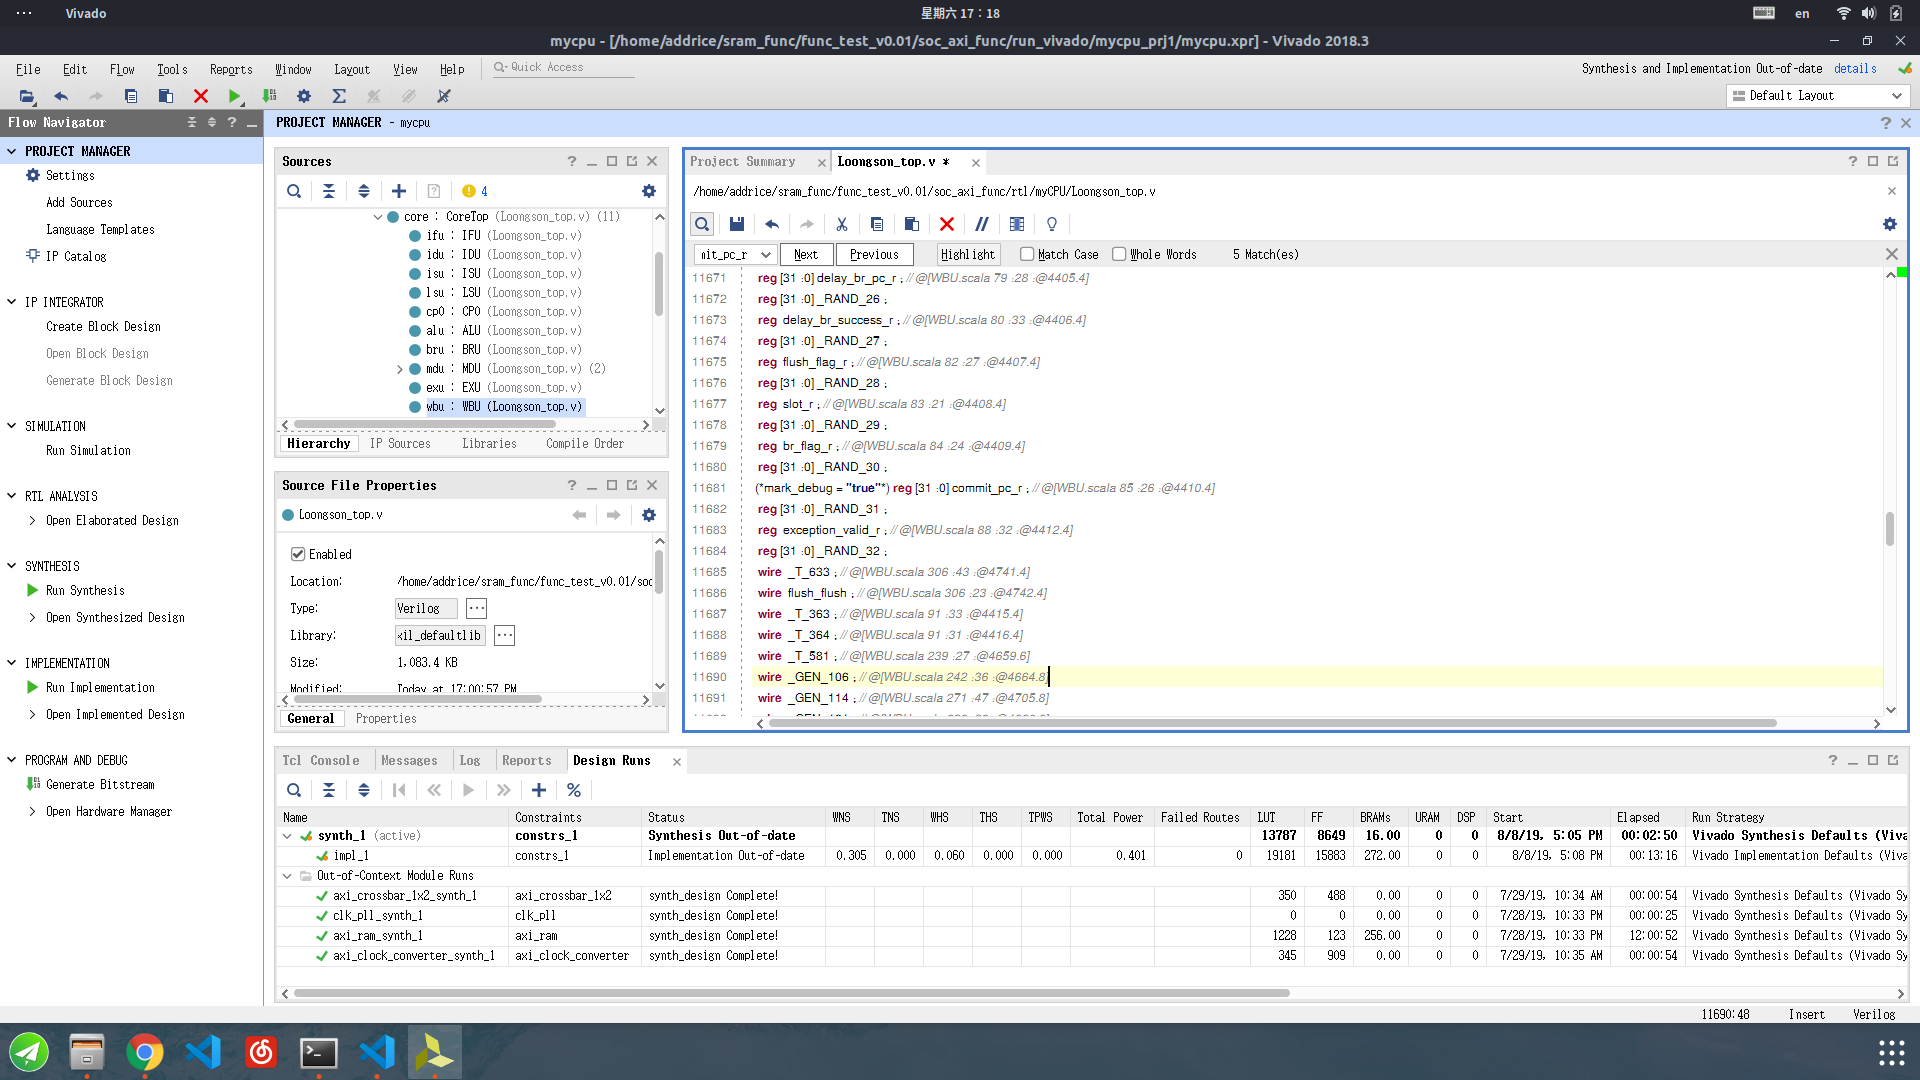
\includegraphics[width=\linewidth]{image/mark_debug_1.png}
\end{figure}

然后综合(Run synthesis),完成后open Synthesized Design,点击Set up Debug,如图所示
\begin{figure}[H]
\centering
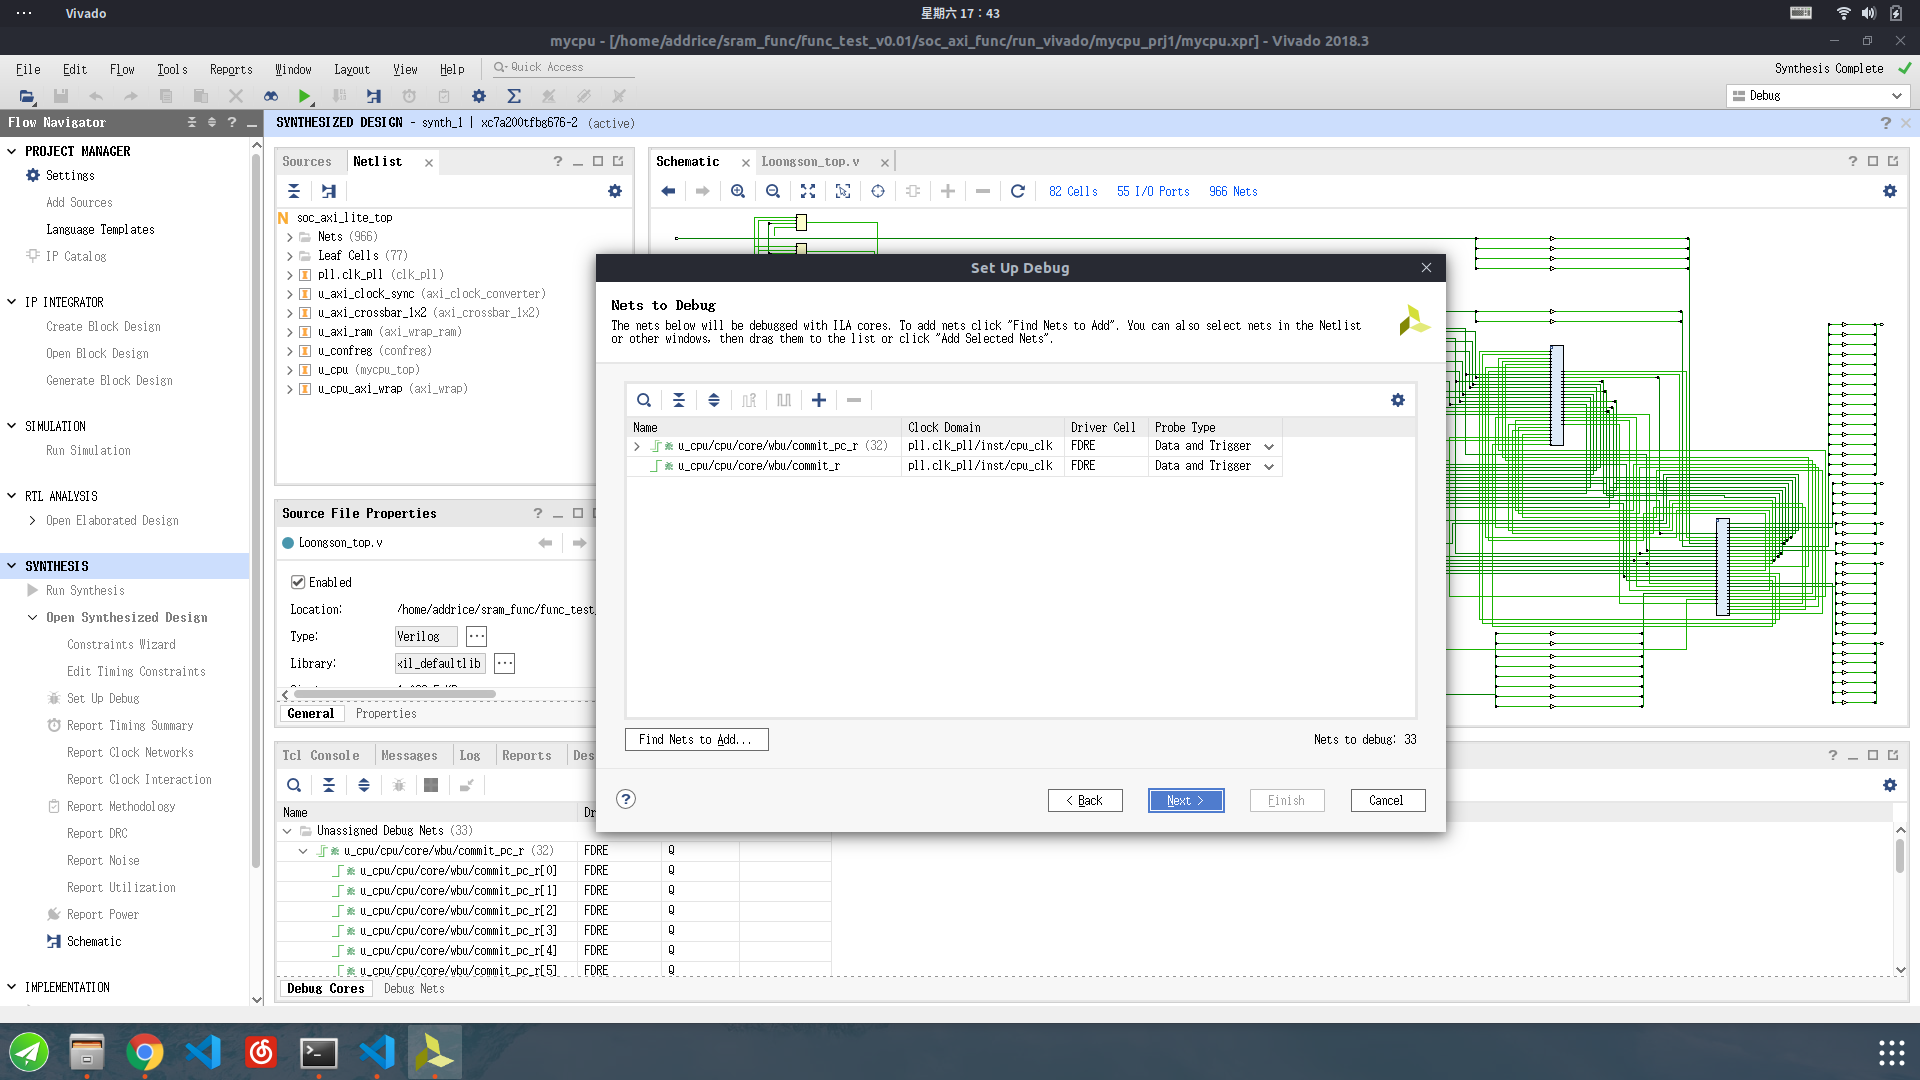
\includegraphics[width=\linewidth]{image/mark_debug_2.png}
\end{figure}
设置过的mark\_debug的信号会显示在其中,点击next,勾选Captrue control和Advanced trigger,如图所示

\begin{figure}[H]
\centering
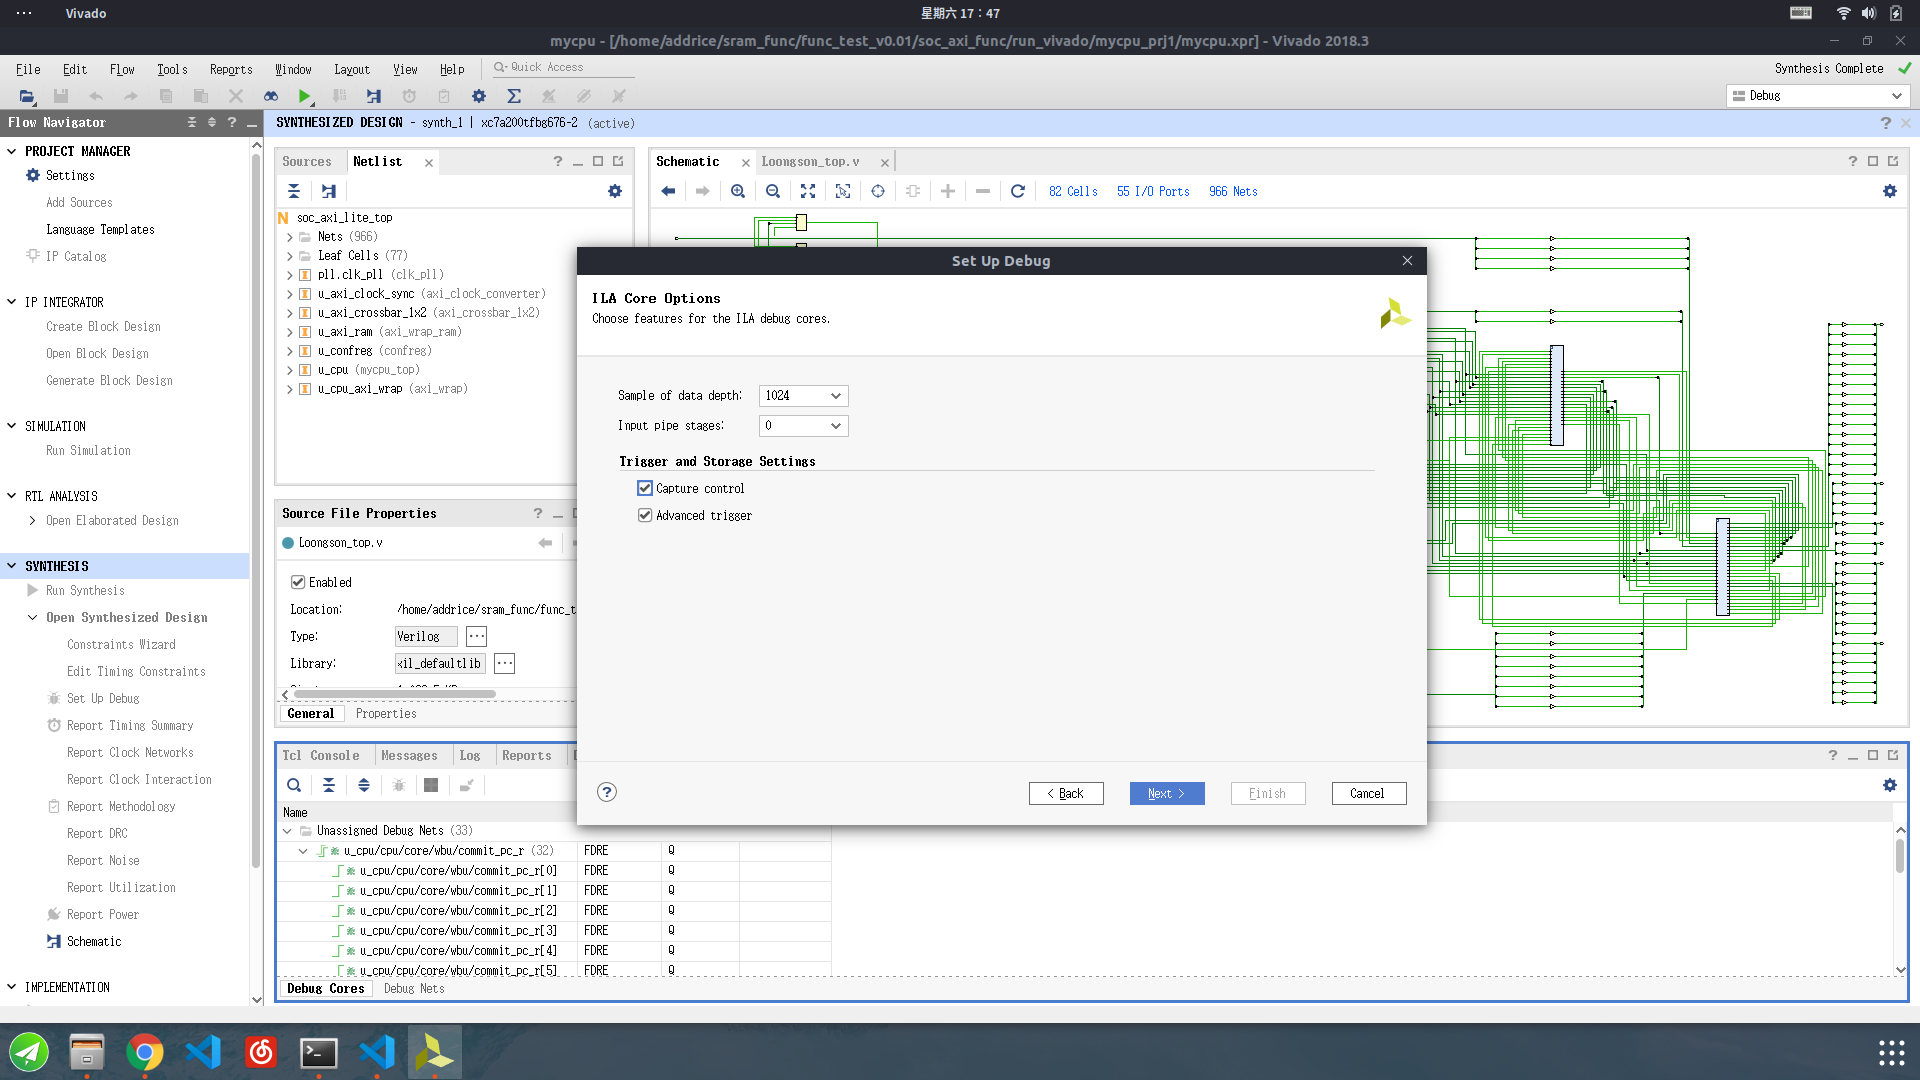
\includegraphics[width=\linewidth]{image/mark_debug_3.png}
\end{figure}
然后一路next完成。这一操作会修改我们的引脚文件,点击生成bitstream,save我们对综合文件的修改,如图所示
\begin{figure}[H]
\centering
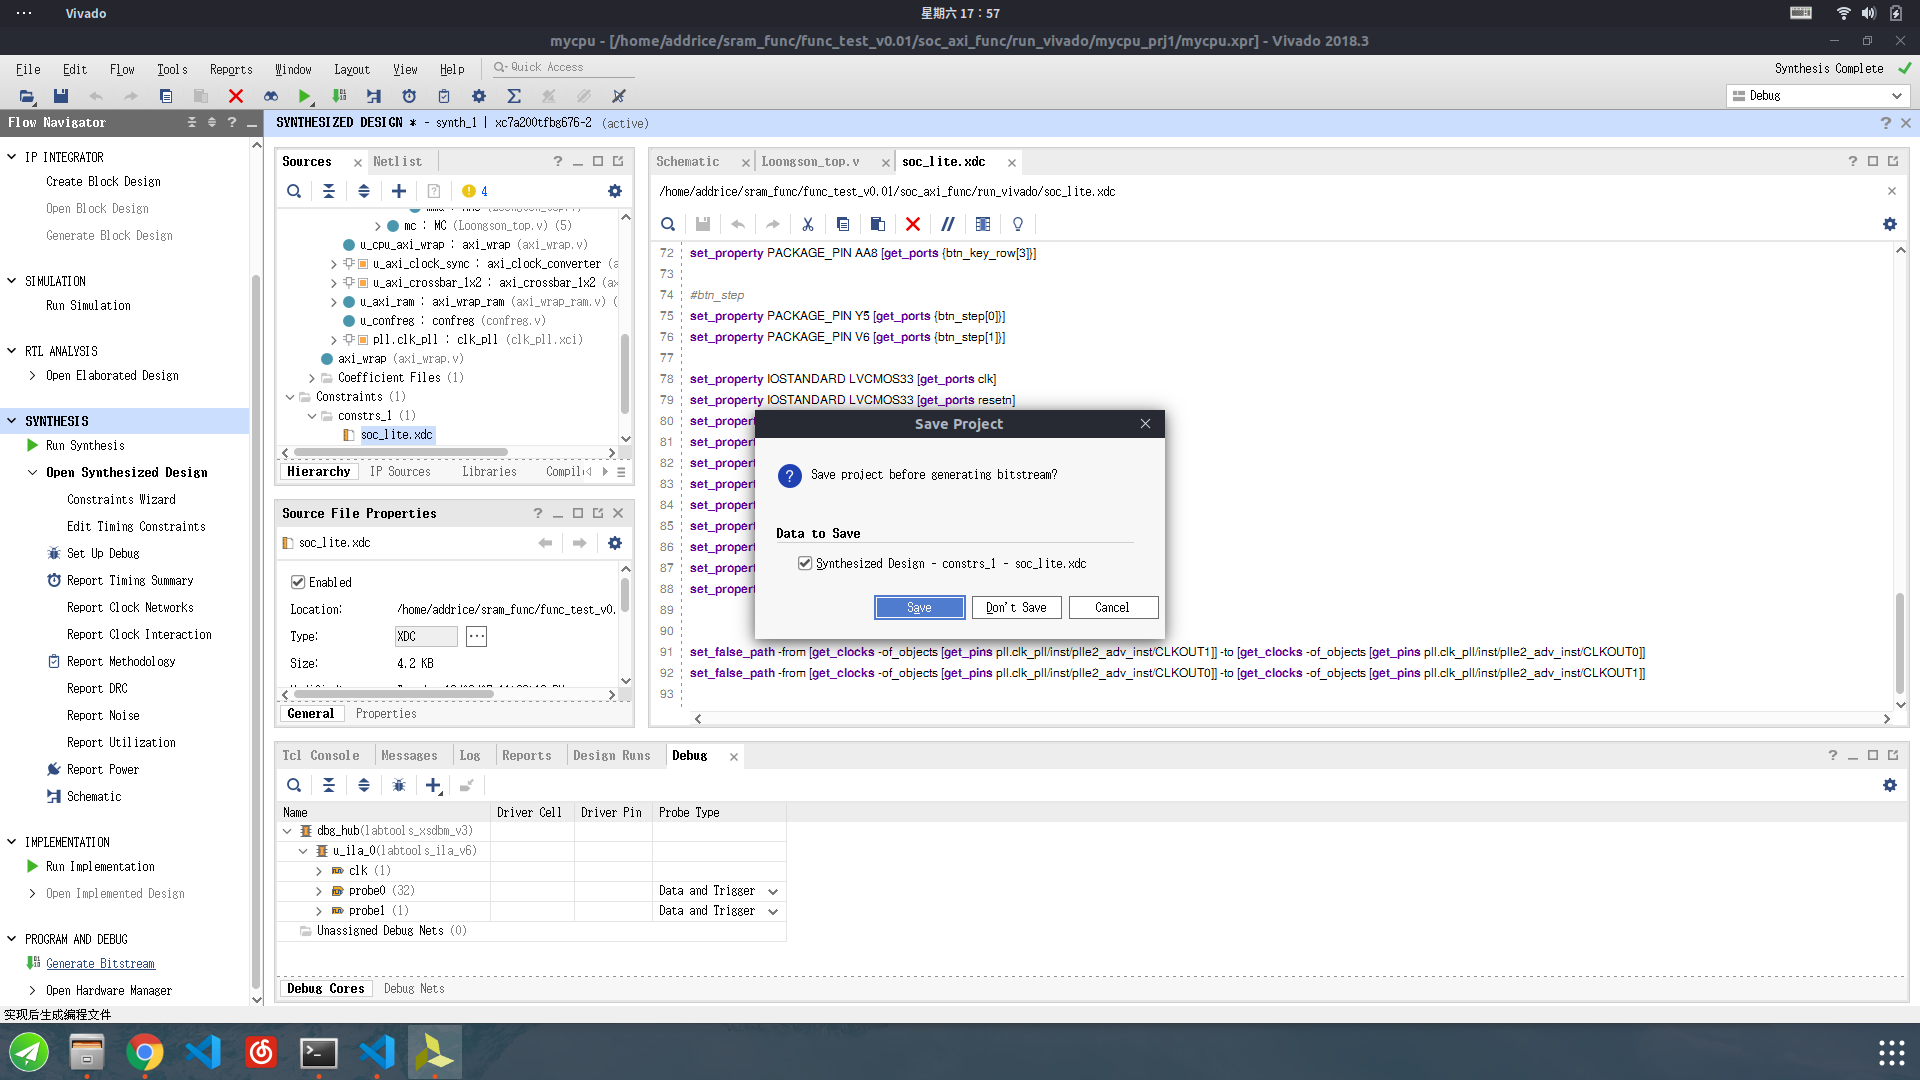
\includegraphics[width=\linewidth]{image/mark_debug_4.png}
\end{figure}
等待bitstream生成完毕上板即可。

\subsubsection{block design上使用system ila}

system ila用来抓取AXI4的信号,相较于用\lstinline!(*mark_debug = "true"*)!,system ila抓取的信号易读性更强,并且可以直接在block design中操作。如下图所示,首先打开block design:

\begin{figure}[H]
\centering
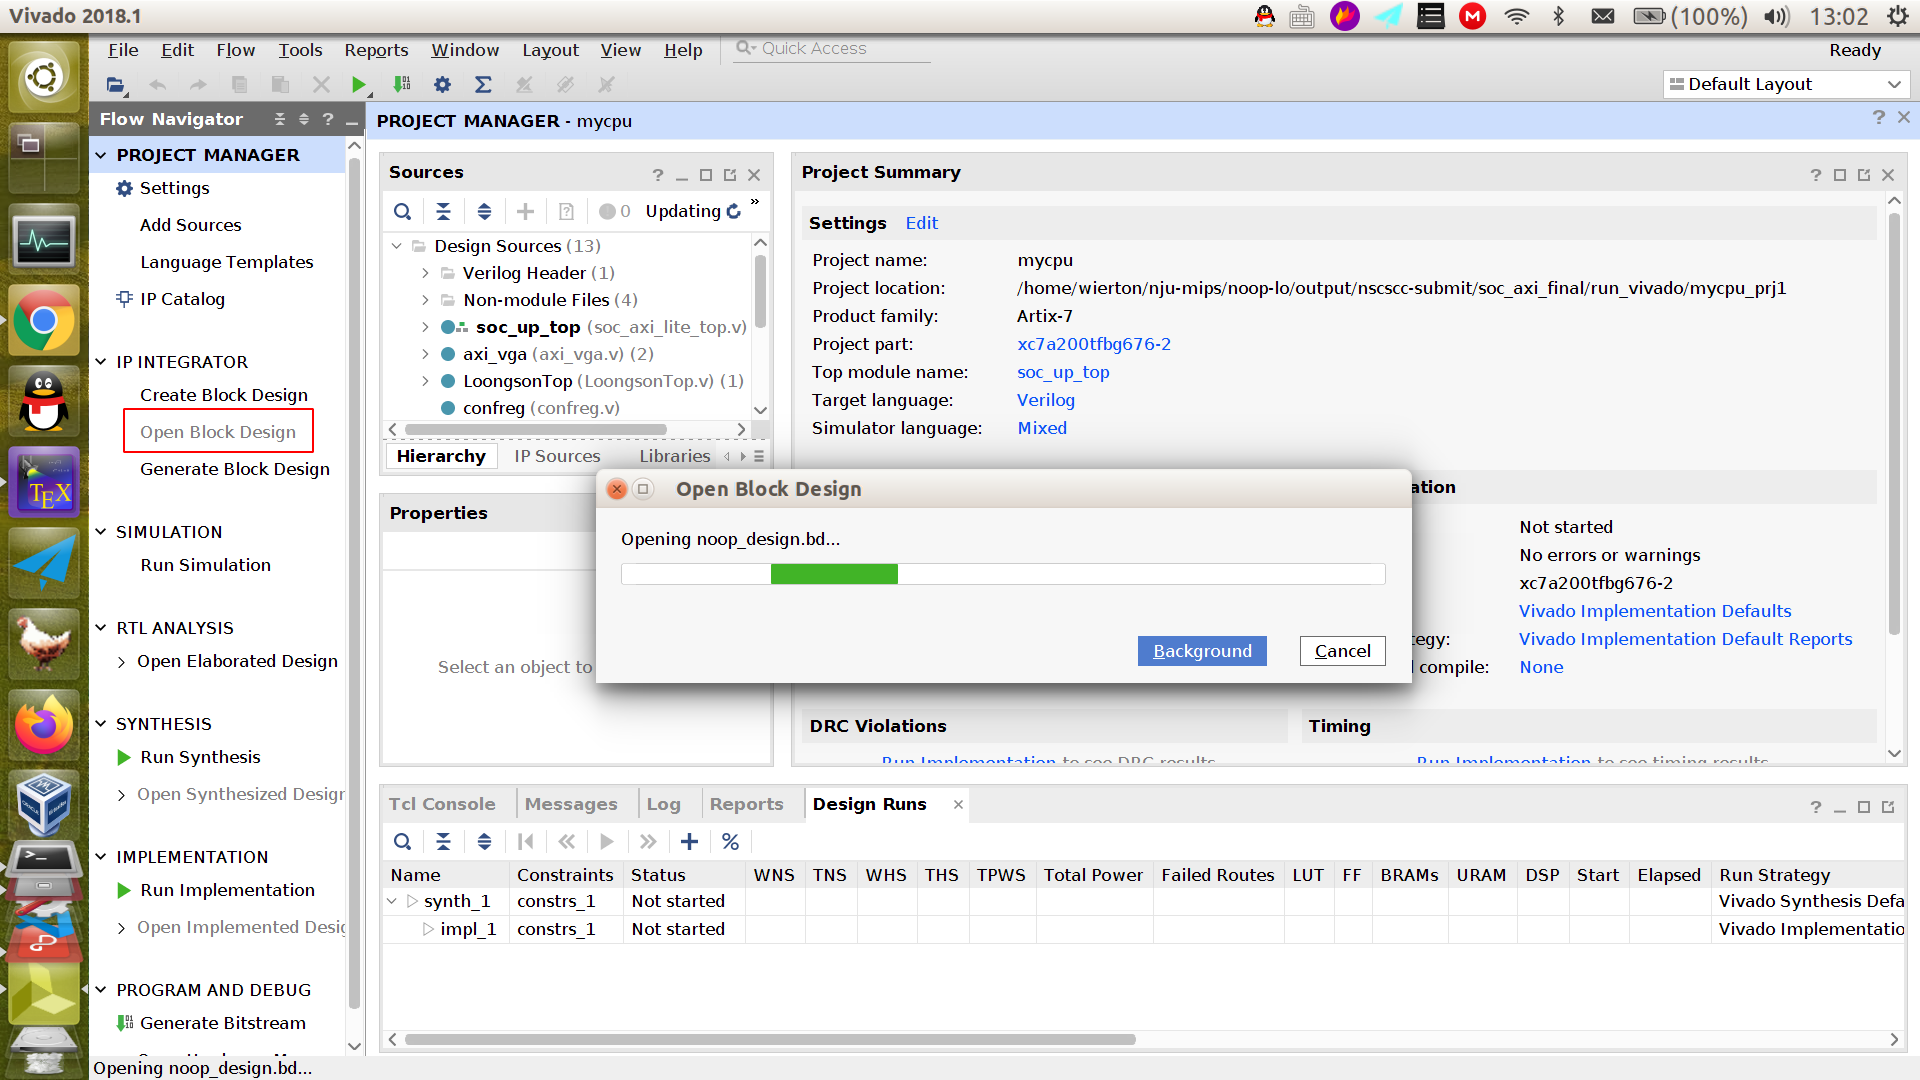
\includegraphics[width=\linewidth]{image/system_ila_1.png}
\end{figure}

然后在block design的面板上右键add IP,搜索system ila:

\begin{figure}[H]
\centering
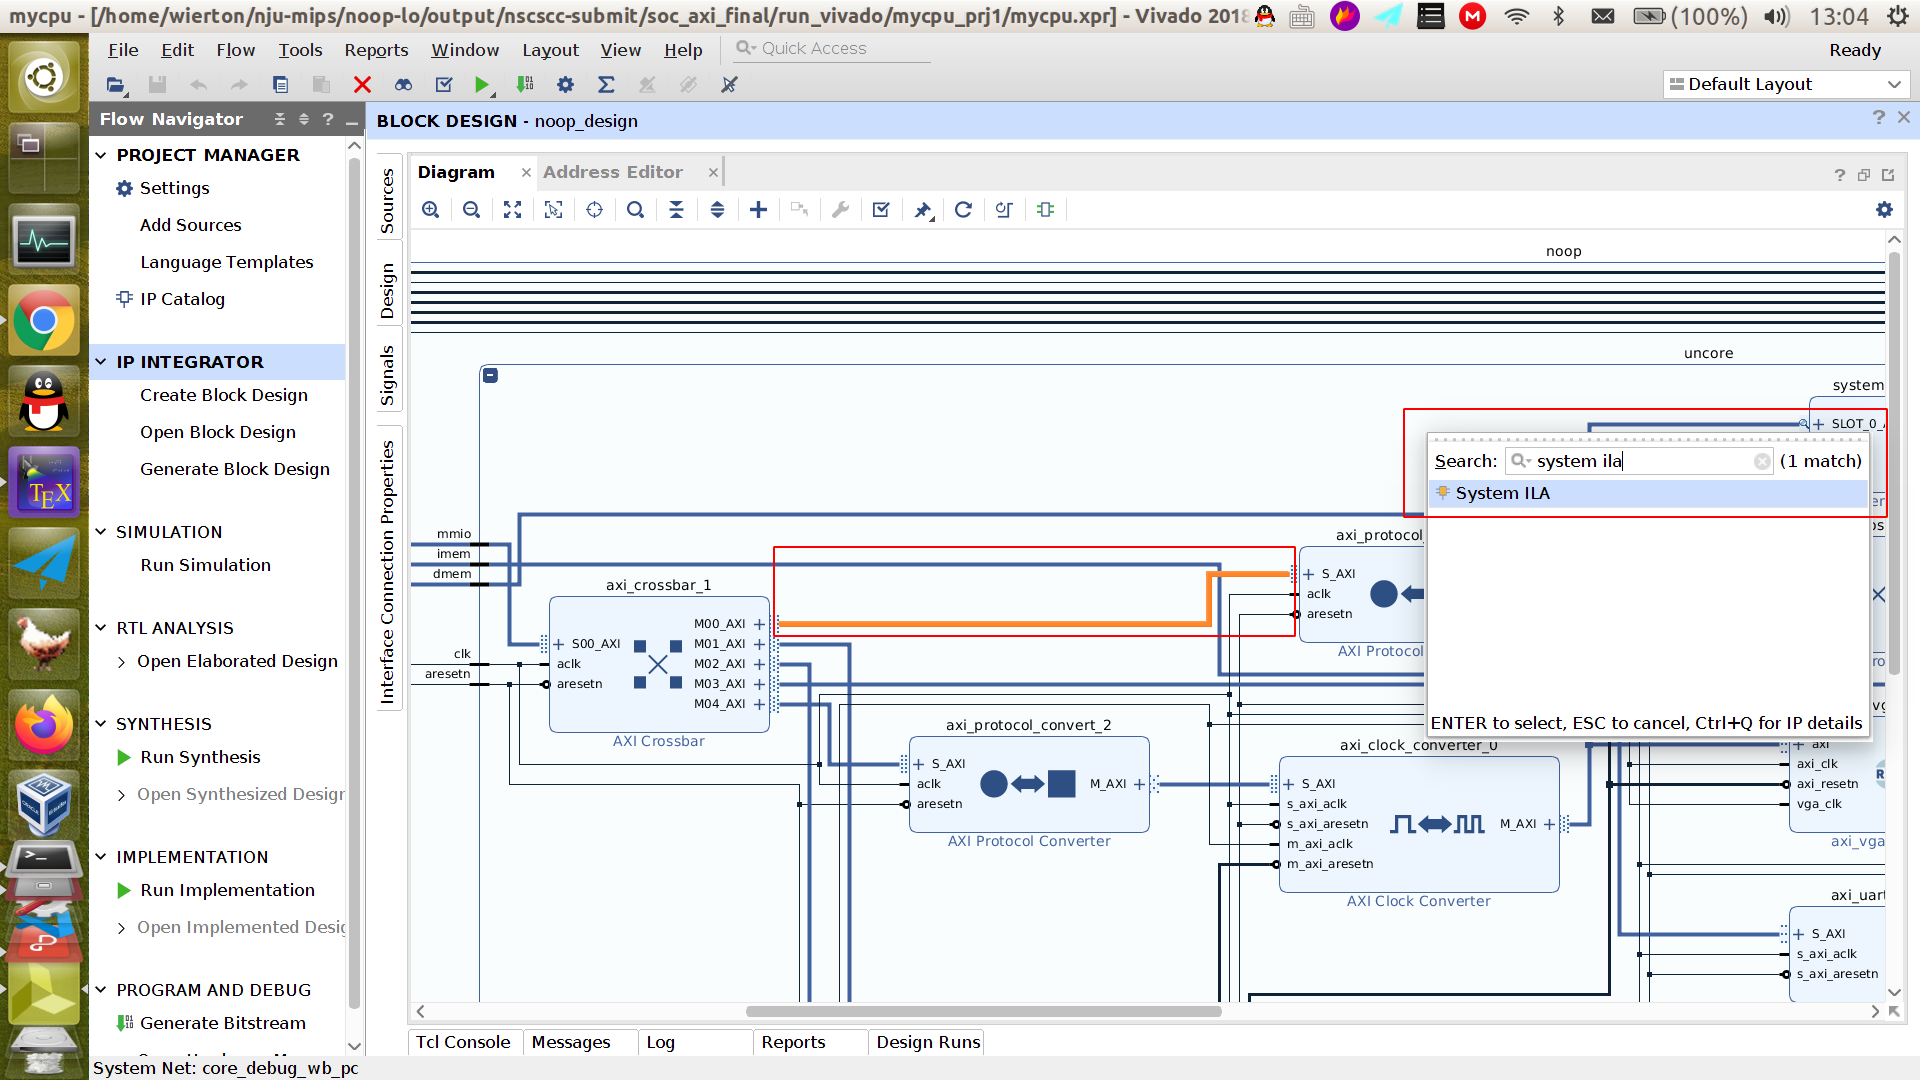
\includegraphics[width=\linewidth]{image/system_ila_2.png}
\end{figure}

最后将system ila的clock、reset和所需要采样的信号连好:
\begin{figure}[H]
\centering
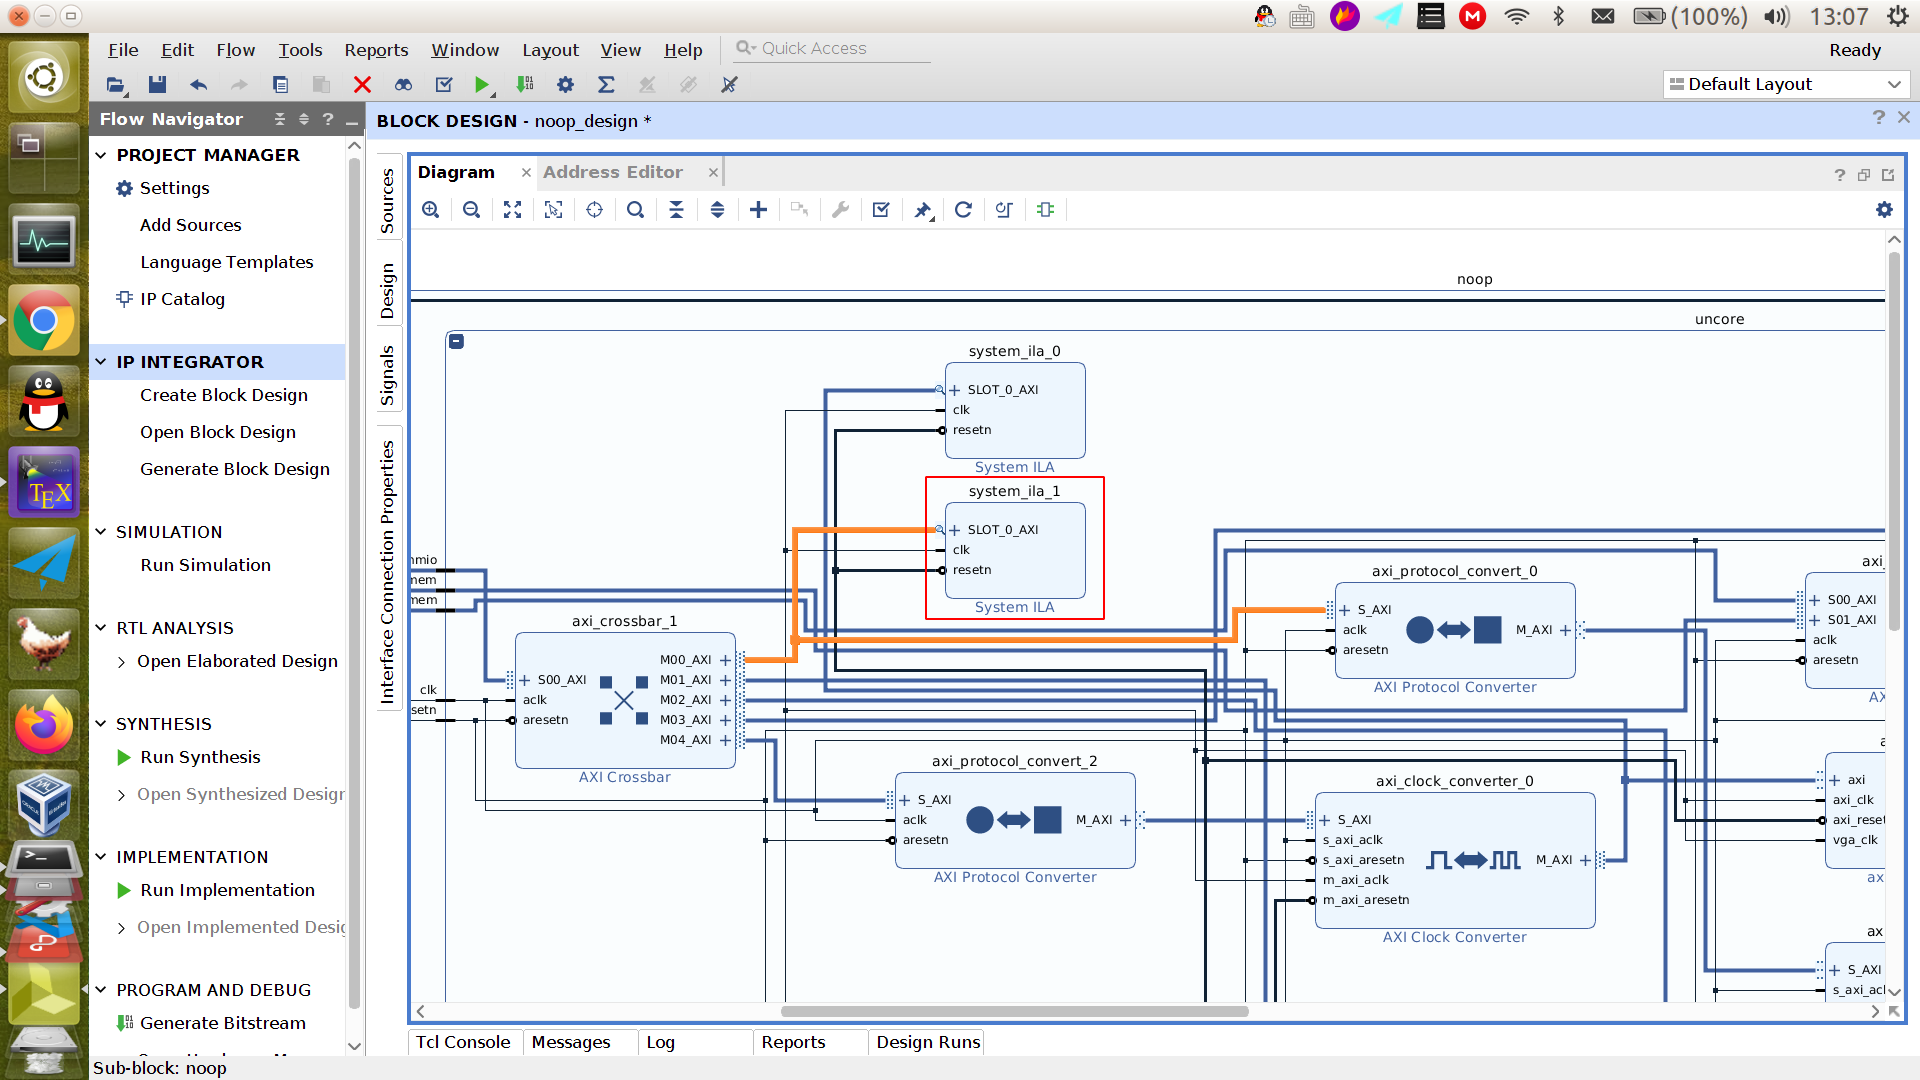
\includegraphics[width=\linewidth]{image/system_ila_3.png}
\end{figure}

后续流程后前面一样,综合上板,然后便会自动进入抓信号的界面。

\section{minilab讲义}
minilab的目的旨在让你能够快速掌握大实验所需的各种工具链,整体还是服务于大实验的。

\subsection{Kconfig}

开始实验前请先下载代码:\lstinline!git clone git@github.com:nju-mips/minilab!,clone下来之后你的文件结构是如下这样:
\begin{lstlisting}
minilab
+-- kconfig
+-- M1
\end{lstlisting}

其中kconfig是linux内核所使用的自动化配置工具,也是这个小实验的重心,不过你并没有必要去研究它的源代码,我们所需要做的是学会去使用它。

下载下来源码之后,进入M1目录,尝试make一下,你会得到如下输出:
\begin{lstlisting}
../kconfig/conf ./Kconfig
*
* This is a simple Kconfig for lab1
*
Algorithm selection
> 1. bubble sort (BUBBLE_SORT) (NEW)
  2. selection sort (SELECTION_SORT) (NEW)
choice[1-2?]:
use printer to print the array (USE_PRINTER) [N/y/?] (NEW)
#
# configuration written to .config
#
../kconfig/conf --syncconfig ./Kconfig
make: *** No rule to make target 'build/main.o', needed by 'build/M1'.  Stop.
\end{lstlisting}

重点是最后一行,\lstinline!No rule to make target 'build/main.o'!,你需要做的第一件事便是打开M1/Makefile.compile,并在里面添加.o文件的规则。为求方便的你可能会将Makefile.compile修改成:
\begin{lstlisting}
build/main.o: src/main.c
  mkdir -p build
  $(CC) -c $(CFLAGS) src/main.c -o build/main.o
\end{lstlisting}
但是这样一来假设项目中有几十个.c文件你便需要写上几十条这样的规则,这种做法是低效且易错的。所幸为了消除这种重复性,Makefile提供了\lstinline!%!语法,它出现在规则中有通配符的含义,你可以用它来只写出一条规则便能自动编译所有的.c。

等你搞定了每个.o的编译规则之后,再次键入\lstinline!make!,你会得到如下的输出:
\begin{lstlisting}
/tmp/ccJtMIec.o: In function `main':
main.c:(.text.startup+0x7): undefined reference to `algo'
main.c:(.text.startup+0x2c): undefined reference to `algo'
main.c:(.text.startup+0x33): undefined reference to `printer'
main.c:(.text.startup+0x58): undefined reference to `printer'
collect2: error: ld returned 1 exit status
Makefile.compile:3: recipe for target 'build/main.o' failed
make: *** [build/main.o] Error 1
\end{lstlisting}

这个错误的含义很明显,链接的时候找不到\lstinline!algo!这个符号,但当你打开bubble\_sort.c的时候,你却能发现\lstinline!algo!赫然躺在文件的末尾。这是为什么,明明定义了这个符号,却还是无法链接?

为了回答这个问题,我们需要引入条件编译这个概念。不过不是指\lstinline!#if xx!这种源代码级别的条件编译,这里的条件编译是指在项目构建的时候,自动根据配置文件来决定需要编译链接哪些文件,这在linux/u-boot/coreutils/busybox中均是常用的技巧。在这里也是类似的,你需要阅读Makefile和src/*.c,并在Makefile中添加适当的代码来让项目可以编译(注意到这里为止不可以修改src目录下的文件)。同时为这个实验我们也设计了相应的测试脚本testall.sh,如果你正确的实现了条件编译,则应该可以通过前六个测试,如下所示:
\begin{lstlisting}
PASS bubble-sort
PASS selection-sort
PASS bubble-sort normal-printer
PASS selection-sort normal-printer
PASS bubble-sort reverse-printer
PASS selection-sort reverse-printer
FAIL reverse-sort normal-printer
FAIL reverse_sort_defconfig
\end{lstlisting}

在搞定了基本的编译之后,你可以尝试执行一下\lstinline!make menuconfig!,并在这之后观察一下M1目录下有什么变化,M1/include下面又有什么变化,这些变化会对这个项目产生什么影响?如果不进行\lstinline!make menuconfig!直接编译,整个项目会发生什么?你可以尝试修改一下Kconfig文件,然后再\lstinline!make menuconfig!,看看有哪些变化。

经历了上述过程,你可能已经理解最后两个测试是要干什么的了。虽然如此,我们还是需要按部就班一下。我们先来讲解一下src和include下的几个源码文件干了一件什么事。在common.h头文件中定义了\lstinline!struct algo!和\lstinline!struct printer!,前者是给一个数组排序,后者是打印一个数组。在main.c里面会声明一个algo,然后用它来进行排序。在bubble\_sort.c和selection\_sort.c里面各自都定义了\lstinline!algo!这个变量,显然如果同时链接这两个文件是会链接失败的。

第七个测试需要你自行添加一个新的排序算法\lstinline!reverse-sort!,它的功能是将输入按从大到小排好序。同时你需要修改Kconfig,添加相应的选项\lstinline!REVERSE_SORT!,并在Makefile里面添加相应的条件编译规则,使得你的修改能够通过第七个测试。

如果你接触过内核的编译,可能会用过\lstinline!make xxx_defconfig!这样的功能。初见时可能感到惊奇,但仔细想一下你可能就知道这个功能是怎么实现的了。第八个测试也是为了测这个功能,具体来说你需要添加一个\lstinline!%_defconfig!的伪目标,这个伪目标会在被执行时去configs目录下将相应的配置文件覆盖到项目当前的配置文件上去。当然配置文件需要你自己准备,具体准备什么样的配置文件可以通过测试你可以通过阅读测试脚本来获得。

\subsection{dts和配置运行linux}

\section{MIPS相关}

\subsection{nju-mips简介}

\subsubsection{CPU Core}
\begin{itemize}
\item 单周期CPU
\item 多周期CPU(考虑信号的阻塞)
\item 一般流水线CPU(标准5段、score board)
\begin{itemize}
\item 长延迟指令(访存,乘除法)
\end{itemize}
\item 高级流水线CPU (分支预测器、ICache、DCache)
\begin{itemize}
\item CP0 (中断、异常)
\item L2 cache
\item TLB
\end{itemize}
\item 乱序流水线CPU
\item 乱序双发射CPU
\end{itemize}

\subsubsection{MIPS standard}
参见手册(\href{run:../manuals/MIPS_Vol1.pdf}{[1]}, \href{run:../manuals/MIPS_Vol2.pdf}{[2]}, \href{run:../manuals/MIPS_Vol3.pdf}{[3]})
\begin{itemize}
\item ALU: 算术运算指令(确定延迟)
  \begin{itemize}
  \item add, addu, addi, addiu, sub, subu, and, andi, clz, or, ori, xor, xori, nor, slt, sltu, slti, sltiu, sll, sllv, srl, srlv, sra, srav, lui, movn, movz
  \item 注意:clz有高效的递归,采用低效方案容易形成关键路径
  \end{itemize}
\item BRU: 分支跳转指令
  \begin{itemize}
  \item beq, bgtz, blez, bltz, bgez, bltzal, bgezal, bne, j, jal, jalr, jr
  \item 注意:所有的分支指令都有延迟槽,即分支后一条指令一定执行
  \end{itemize}
\item LSU: 访存指令(不定延迟)
  \begin{itemize}
  \item 对齐访存指令: lb, lbu, lh, lhu, lw, sb, sh, sw
  \item 不对齐访存指令: lwl, lwr, swl, swr
  \item 原子性读写指令: ll, sc
  \end{itemize}
\item MDU: 乘除法指令(长延迟)
  \begin{itemize}
  \item mul, mult, multu, div, divu, mfhi, mflo, mthi, mtlo
  \item 建议:hi和lo寄存器随通用寄存器一起进行转发,如果单独放在MDU里面,后续高级流水线的时候需要两套处理方案
  \end{itemize}
\item PRU: 特权指令(该单元包括CP0和TLB),重点看\href{run:../manuals/MIPS_Vol3.pdf}{[3]}
  \begin{itemize}
  \item syscall: 发起系统调用的指令
  \item eret: 系统调用执行完从内核态返回用户态的指令
  \item mfc0: cp0有自己的一套标准规定的寄存器,这条指令用于读cp0寄存器到一般寄存器
  \item mtc0: 用于将一般寄存器的值写入cp0
  \item tlbp: 用于查询一个虚拟地址的页表项是否存在
  \item tlbr: 用于读取一个页表项(cp0维护虚拟地址到物理地址的映射,形式有标准规定)
  \item tlbw: 用于写入一个页表项
  \item tlbwr: 由硬件随机淘汰一个旧页表项,并将新表项写入
  \item cache: 用于控制cache,包括将cache的一行写回,标记为无效等操作
  \item pref: 内存预取指令,用于加速,具体实现的时候可以什么都不做
  \item sync: 多核之间同步的指令,单核可以什么都不做
  \item break: 抛异常就行了
  \item tlt, tge, tltu, tgeu, tlti, teqi, tgei, tnei, tltiu, tgeiu, tne, teq: 自陷指令,条件满足的时候让cpu停住,不要抛异常了,直接在开发板上点个灯,正常执行是不会有这条指令的
  \end{itemize}
\item CP0: 0号协处理器
  \begin{itemize}
  \item 维护页目录,页目录缺失由操作系统回填,硬件抛异常就行了
  \item 维护cp0寄存器,下述以建议的实现顺序排序:
    \begin{itemize}
    \item status, cause, epc (实现系统调用必须)
	\item badvaddr (实现异常必须,用于指示最后一个出错的访存地址)
	\item index, pagemask, context, entry\_lo0, entry\_lo1, entry\_hi (实现虚存必须)
	\item count, compare (实现时间中断必须)
	\item prid, config, config1 (运行u-boot和linux必需)
	\item base (可选,旧标准内没有,用于调整异常向量表的基址,缺省为0xbfc00000)
      \begin{itemize}
	  \item cpu启动时也是0xbfc00000,所以异常向量一般需要后期写入
      \end{itemize}
    \end{itemize}
  \end{itemize}
\item CP0寄存器的布局
  \begin{itemize}
  \item 寻址: (待续)
  \end{itemize}
\item CP1:1号协处理器
  \begin{itemize}
  \item 关于浮点数的,可以使用IP核,需要实现的指令数不多,可在后续提升时实现
  \end{itemize}
\end{itemize}

\subsubsection{CPU uncore}

\begin{itemize}
\item \href{run:../manuals/AXI4.pdf}{[AXI4]}: 最常用的核外总线协议
  \begin{itemize}
  \item 几乎绝大多数硬件的IP核都会使用这个协议
  \item AXI4lite, 简化版的AXI4,但是不支持burst传输,一开始可以用这个
  \end{itemize}
\item Uartlite (用axi4-uartlite的IP核就行,无需自行实现)
  \begin{itemize}
  \item 最简单的串口协议
  \item 连接串口的简单教程\ref{minicom}
  \end{itemize}
\item Emaclite (不需要深入理解、用就可以了)
  \begin{itemize}
  \item 最简单的网口协议,vivado里面有IP核,u-boot和linux里面均有驱动
  \end{itemize}
\item SPI flash
  \begin{itemize}
  \item 注意SPI仅为通信协议,实际想要读写flash,需通过SPI的IP核将命令发送给flash芯片,关于flash的命令,这里不推荐任何手册。其状态机过于复杂,这里不建议花太多时间
  \item 如果想要使用flash,请先将linux跑起来,linux里有驱动,无需再自己实现
  \end{itemize}
\item PS/2
  \begin{itemize}
  \item 注意,PS/2也仅是通信协议,用于与键盘和鼠标交互,实际读取键盘和鼠标还需基于PS/2发送命令
  \item PS/2在vivado里面有IP核,在linux里面有驱动,如果可以跑通linux,那么使用PS/2是比较容易的
  \end{itemize}
\item VGA (用往届的就可以了)
  \begin{itemize}
  \item 数电课的VGA控制器包装成AXI4控制接口
  \end{itemize}
\item BlockRAM、RAM
  \begin{itemize}
  \item 片上资源,BlockRAM是读写均同步,适合用来做cache
  \item RAM,写同步,读异步,适合用来做register
  \end{itemize}
\end{itemize}

\subsubsection{SOC构建与调试常用的工具链}
\begin{itemize}
\item Makefile \ref{Makefile}
  \begin{itemize}
  \item 用于将一键化各种功能
  \end{itemize}
\item tcl脚本
  \begin{itemize}
  \item vivado的自动化脚本,可以调用vivado的功能
  \item 如果需要一键创建vivado项目,这个是常用的工具
    \begin{itemize}
    \item vivado可以将当前项目导出到tcl脚本
    \end{itemize}
  \end{itemize}
\item block design
  \begin{itemize}
  \item 用图形界面来连接模块和IP核
  \end{itemize}
\item verilator \ref{verilator}
  \begin{itemize}
  \item verilog的模拟器,非常快,可以方便你们回归测试
  \item 到后期,用到IP核的时候,还需要用vivado的仿真工具
  \item 样例工程在`examples/1.Makefile-chisel-sample`中
  \end{itemize}
\item chisel
  \begin{itemize}
  \item 高级硬件描述语言
  \item 样例工程在`examples/1.Makefile-chisel-sample`中
  \end{itemize}
\item ILA
  \begin{itemize}
  \item 调试的终极大招,可以在板上电路中采样信号
  \end{itemize}
\end{itemize}

\subsection{关于PRU的一些实现细节}

PRU全称PRiviledged Unit,用来实现CP0和TLB。

\subsubsection{必要的cache指令}

mips不同于x86,ICache与DCache之间的一致性需要通过cache指令来维护。但是具体实现的时候无需把cache指令的所有功能都实现一遍,cache指令的某些操作码并没有被使用过。表\ref{tab:cache_inst}记录了linux和u-boot中所使用的cache指令。

\begin{table}[H]
\centering
\begin{tabular}{|c|c|c|c|c|}
\hline
cache指令 & 操作码 & 作用的cache & 使用范围 & 具体功能 \\\hline
\hline
\lstinline!cache 0x00, [addr]! & \lstinline!5b000'00! & 指令cache & linux & \\\hline
\lstinline!cache 0x08, [addr]! & \lstinline!5b010'00! & 指令cache & linux & \\\hline
\lstinline!cache 0x10, [addr]! & \lstinline!5b100'00! & 指令cache & linux+u-boot & \\\hline
\lstinline!cache 0x14, [addr]! & \lstinline!5b101'00! & 指令cache & linux & \\\hline
\hline
\lstinline!cache 0x01, [addr]! & \lstinline!5b000'01! & 数据cache & linux & \\\hline
\lstinline!cache 0x09, [addr]! & \lstinline!5b010'01! & 数据cache & linux & \\\hline
\lstinline!cache 0x15, [addr]! & \lstinline!5b101'01! & 数据cache & linux+u-boot & \\\hline
\hline
\lstinline!cache 0x03, [addr]! & \lstinline!5b000'11! & L2 cache & linux & \\\hline
\lstinline!cache 0x07, [addr]! & \lstinline!5b001'11! & L2 cache & linux & \\\hline
\lstinline!cache 0x13, [addr]! & \lstinline!5b100'11! & L2 cache & linux & \\\hline
\lstinline!cache 0x17, [addr]! & \lstinline!5b101'11! & L2 cache & linux & \\\hline
\lstinline!cache 0x0b, [addr]! & \lstinline!5b010'11! & L2 cache & linux & \\\hline
\end{tabular}
\caption{常用cache指令}
\label{tab:cache_inst}
\end{table}

\subsubsection{异常实现的注意点}

关于异常,最需要注意的一点是它和异常码不是一一对应的,异常跳转入口可以视为是由异常和异常码共同决定的:

\begin{table}[H]
\centering
\begin{tabular}{|c|c|}
\hline
异常 & 会产生的异常码 \\\hline
TLB Refill Exception & TLBL, TLBS \\\hline
TLB Invalid Exception & TLBL, TLBS \\\hline
TLB Modified Exception & TLBMod \\\hline
\end{tabular}
\caption{需要注意的异常和异常码}
\end{table}

下述为处理异常发生时如何跳转的代码,原版在nemu-mips32/src/cpu/cpu.c中:
\begin{lstlisting}[language=c]
void launch_exception(int exception, int excode) {
  // 注意,异常和异常码不是一一对应的
  uint32_t vecOff = 0;
  if (cpu.cp0.status.EXL == 0) {
    if (cpu.last_instr_in_delayslot) {
      cpu.cp0.epc = cpu.pc - 4; // 跳转指令的地址
      cpu.cp0.cause.BD = 1;
    } else {
      cpu.cp0.epc = cpu.pc;     // 最后执行的指令的地址
      cpu.cp0.cause.BD = 0;
    }

    // 这里计算异常入口地址的偏移量
    if (exception == EX_TLB_REFILL)
      vecOff = 0x000;
    else if (excode == EXC_INTR && cpu.cp0.cause.IV == 1)
      vecOff = 0x200;
    else
      vecOff = 0x180;
  } else {
    // 注意这里不设置epc
    vecOff = 0x180;
  }

  cpu.cp0.cause.ExcCode = code;
  cpu.cp0.status.EXL = 1;
  // 注意这里,异常跳转地址的计算方式是[基址+偏移量]
  if (cpu.cp0.status.BEV == 1) {
    cpu.br_target = 0xbfc00200 + vecOff;
  } else {
    cpu.br_target = 0x80000000 + vecOff;
  }
}
\end{lstlisting}

\subsubsection{tlb实现细节}

关于查询tlb的过程中如何发起异常,可以参见nemu-mips32/src/cpu/mmu.c,下述代码对原版做了简化。

\begin{lstlisting}[language=c]
void tlb_exception(int ex, int code, vaddr_t vaddr, unsigned asid) {
  cpu.cp0.badvaddr = vaddr;
  cpu.cp0.context.BadVPN2 = vaddr >> 13;
  cpu.cp0.entry_hi.vpn = vaddr >> 13;
  cpu.cp0.entry_hi.asid = asid;
  launch_exception(ex, code);
}

vaddr_t page_translate(vaddr_t vaddr, int rwbit) {
  uint32_t excode = rwbit == MMU_LOAD ? EXC_TLBL : EXC_TLBS;
  uint32_t va_31_13 = (vaddr & ~0x1FFF) >> 13;
  for (int i = 0; i < NR_TLB_ENTRY; i++) {
    uint32_t mask = tlb[i].pagemask;
    assert(mask == 0 || (mask | (mask + 1)) == 0);
    bool match = (tlb[i].vpn & ~mask) == (va_31_13 & ~mask) &&
                 (tlb[i].g || tlb[i].asid == cpu.cp0.entry_hi.asid);
    if (!match) continue;

    bool EvenOddBit = vaddr & ((mask + 1) << 12);
    /* match the vpn and asid */
    tlb_phyn_t *phyn = EvenOddBit ? &(tlb[i].p1) : &(tlb[i].p0);
    if (phyn->v == 0) {
      tlb_exception(EX_TLB_INVALID, excode, vaddr, tlb[i].asid);
      return -1u;
    } else if (phyn->d == 0 && rwbit == MMU_STORE) {
      tlb_exception(EX_TLB_MODIFIED, EXC_TLBM, vaddr, tlb[i].asid);
      return -1u;
    } else {
      // # pfn_PABITS-1-12..0 corresponds to pa_PABITS-1..12
      //
      // pa ← pfn_PABITS-1-12..EvenOddBit-12 || va_EvenOddBit-1..0
      // case TLB[i].Mask
      //  2#0000000000000000: EvenOddBit ← 12
      //  2#0000000000000011: EvenOddBit ← 14
      //  2#0000000000001111: EvenOddBit ← 16
      // endcase

      uint32_t highbits = (phyn->pfn & ~mask) << 12;
      uint32_t lowbits = vaddr & (((mask + 1) << 12) - 1);
      return highbits | lowbits;
    }
  }

  tlb_exception(EX_TLB_REFILL, excode, vaddr, cpu.cp0.entry_hi.asid);
  return -1u;
}
\end{lstlisting}

\subsection{外设地址段}

\begin{table}[H]
\centering
\begin{tabular}{|c|c|}
\hline
 地址段 & 外设 \\\hline
\lstinline!0x80000000 - 0x8fffffff! & DDR (cached) \\\hline
\lstinline!0xa0000000 - 0xafffffff! & DDR (uncached) \\\hline
\lstinline!0xb0000000 - 0xb0000fff! & nemu GPIO trap \\\hline
\lstinline!0xb0002000 - 0xb0002fff! & nemu rtc \\\hline
\lstinline!0xb0003000 - 0xb0003fff! & nemu screen config \\\hline
\lstinline!0xb0400000 - 0xb04fffff! & nemu video memory \\\hline
\lstinline!0xbfc00000 - 0xbfcfffff! & SRAM(用于存放引导程序) \\\hline
\lstinline!0xbfe50000 - 0xbfe50fff! & xilinx uartlite serial \\\hline
\lstinline!0xbfe80000 - 0xbfe80fff! & xilinx spi flash \\\hline
\lstinline!0xbfe94000 - 0xbfe94fff! & nemu Keyboard \\\hline
\lstinline!0xbfe95000 - 0xbfe95fff! & npc PerfCounter \\\hline
\lstinline!0xbfe96000 - 0xbfe95fff! & PS/2 keyboard \\\hline
\lstinline!0xbff00000 - 0xbff0ffff! & xilinx emaclite \\\hline
\end{tabular}
\end{table}



\subsection{CLZ的递归高效实现}
\subsubsection{函数版本}

\begin{lstlisting}
object CountLeadingZeros32 {
  def apply(in: UInt):UInt = {
    val out = Wire(Vec(5, Bool()))

    out(4) := in(31, 16) === 0.U(16.W)

    val val16 = Mux(out(4), in(15, 0), in(31, 16))
    out(3) := val16(15, 8) === 0.U(8.W)

    val val8  = Mux(out(3), val16(7, 0), val16(15, 8))
    out(2) := val8(7, 4) === 0.U(4.W)

    val val4  = Mux(out(2), val8(3, 0), val8(7, 4))
    out(1) := val4(3, 2) === 0.U(2.W)

    out(0) := Mux(out(1), ~val4(1), ~val4(3))

    Mux(in === 0.U, 32.U, out.asUInt)
  }
}
\end{lstlisting}

\subsubsection{模块版本(不建议使用)}

\begin{lstlisting}
class CountLeadingZeros32 extends Module {
  val io = IO(new Bundle {
    val in = Input(UInt(32.W))
    val out = Input(UInt(32.W))
  })

  val tmp = Wire(Vec(5, Bool()))
  tmp(4) := io.in(31, 16) === 0.U(16.W)

  val val16 = Mux(tmp(4), io.in(15, 0), io.in(31, 16))
  tmp(3) := val16(15, 8) === 0.U(8.W)

  val val8  = Mux(tmp(3), val16(7, 0), val16(15, 8))
  tmp(2) := val8(7, 4) === 0.U(4.W)

  val val4  = Mux(tmp(2), val8(3, 0), val8(7, 4))
  tmp(1) := val4(3, 2) === 0.U(2.W)

  tmp(0) := Mux(tmp(1), ~val4(1), ~val4(3))

  io.out := Mux(io.in === 0.U, 32.U, tmp.asUInt)
}
\end{lstlisting}

\section{相关项目说明}

写在前面,所有的相关项目只做概述性说明。由于项目本身也在经常重构,一些整理的内容到后期可能就不对了,同时对于计算机系统综合实验的同学而言,看代码也是一个必由之路。

\subsection{测试相关}

\subsubsection{insttest}
这个项目是从龙芯的测试集和清华的测试集里扒出来的,用于进行单指令测试。需要注意的一点是,一旦开始流水线设计,单指令测试只能验证最基本的正确性,由于流水线的指令间并行性,不同的指令流可能会导致不同的状态机切换,因而造成单指令测试所无法触发的bug。
\subsubsection{tlbtest}
这个是从龙芯的测试集中扒出来的,用于进行tlb的测试,需要注意的是,这个测试并不完备,完备的测试还是需要运行linux这样的workload。
\subsubsection{nexus-am/tests/cputest}
基于AM的一些简单测试,继承自PA,可以测试一些简单的workload
\subsubsection{nexus-am/apps/coremark}
基于AM的评分程序,workload中等。
\subsubsection{nexus-am/apps/microbench}
基于AM的大型workload,很多流水线bug可以在这个测试下暴露出来,需要予以重视。这个测试由于运行时间过长,大部分时候可能只能在板上测试,届时可能需要大量使用ILA。一般普通流水线的microbench跑分可以到达200-300分,这个成绩大概是决赛的垫底成绩,如果想进龙芯杯决赛,还需要多多优化。

\subsection{运行linux相关}

运行linux相关的几个项目都使用了Kconfig进行配置,在nju-mips的几个仓库里面,均已经准备好了针对noop的配置文件,在编译前通过\lstinline!make noop_defconfig!即可初始化配置,除此以外还可以通过\lstinline!make menuconfig!来进行手动配置。后期可以肯定还需要对linux进行裁剪适配,手动配置应是必须掌握的技能之一。

除了Kconfig,u-boot和linux还使用dts文件来描述soc所能访问的外设。dts文件的语法可以百度,如果想了解某个外设的dts文件怎么写,可以查询xilinx的官网。比如加一个emaclite硬件,可以访问\url{https://xilinx-wiki.atlassian.net/wiki/spaces/A/pages/18842124/U-Boot+Ethernet+Driver}查看具体流程

\subsubsection{u-boot}

u-boot是一个引导程序,一般建议直接烧录在SOC的sram中,用于引导程序。\textcolor{red}{其正确运行依赖于cp0里面的cache指令}。u-boot中包含丰富的驱动,结合vivado丰富的IP核,使得我们可以简单组合一下uncore和配置一下u-boot就能让干成很多事情。比如从网口加载内核并执行。

u-boot的(重要)目录结构如下:
\begin{lstlisting}
u-boot
+-- board/                     # 初始化板子的代码
+-- drivers/                   # 各种驱动代码
|   +-- serial/
|   |   +-- serial_xuartlite.c # xilinx uartlite驱动,有大小端bug,nju-mips上已修复
|   +-- spi/
|   |   +-- xilinx_spi.c       # spi驱动,与flash相关
|   +-- net/
|       +-- xilinx_emaclite.c  # xilinx的emaclite驱动
+-- arch/
|   +-- mips/
|       +-- mach-noop/         # 移植到noop所需目录
|       +-- dts/
|           +-- noop.dts       # 描述noop soc外设的文件
+-- configs/
    +-- noop_defconfig         # noop的配置文件
\end{lstlisting}

\subsubsection{linux}

这个项目是linux的内核,无需多言。\textcolor{red}{请务必注意的一点是,在mips里面异常和异常号不是一一对应的,同一个异常号对应的异常可能实际走的异常入口并不一样,这一点手册没有很好的说明},除此以外如果linux运行不起来请着重检查cp0和tlb,尤其是tlb。

linux的重要目录结构如下:
\begin{lstlisting}
u-boot
+-- drivers/                      # 各种驱动代码
|   +-- tty/
|   |   +-- serial/
|   |       +-- uartlite.c        # uartlite驱动,mainline有bug,已修复
|   +-- spi/
|   |   +-- spi-xilinx.c          # spi驱动,与flash相关
|   +-- net/
|       +-- etherlite/
|           +-- xilinx/
|               +-- xilinx_emaclite.c
|               +-- xilinx_axinet.c
+-- arch/
    +-- mips/
        +-- noop/                 # 移植到noop所需目录
        +-- boot/
        |   +-- dts/
        |       +-- noop/
        |           +-- noop.dts  # 描述noop soc外设的文件
        +-- configs/
            +-- noop_defconfig    # noop的配置文件
\end{lstlisting}

关于如何驱动外设,这里需要额外说明一下。假设现在需要驱动uartlite这个外设,首先需要运行\lstinline$make menuconfig$将这个外设的驱动开启,然后需要进入noop.dts文件中,添加对uartlite这个外设的描述,最后在启动时也就有这个外设了。那么这个外设怎么访问呢?还是以uartlite为例,我们打开其驱动文件uartlite.c,会发现有这样几行:
\begin{lstlisting}[language=c]
#define ULITE_NAME		"ttyUL"
#define ULITE_MAJOR		204
#define ULITE_MINOR		187

static struct uart_driver ulite_uart_driver = {
	.owner		= THIS_MODULE,
	.driver_name	= "uartlite",
	.dev_name	= ULITE_NAME,
	.major		= ULITE_MAJOR,
	.minor		= ULITE_MINOR,
	.nr		= ULITE_NR_UARTS,
#ifdef CONFIG_SERIAL_UARTLITE_CONSOLE
	.cons		= &ulite_console,
#endif
};
\end{lstlisting}

这几行意味这,uartlite这个外设被检测到以后,会在/dev下生成/dev/ttyUL这个设备文件,其对应的设备号是\lstinline!204, 187!,如果有多个外设,则他们从0开始排序,如/dev/ttyUL0、/dev/ttyUL1、...。

有时候你会在百度的时候发现有些linux启动的时候会有参数\lstinline!root=/dev/mmcblock!,这就意味这有一个外设名为mmcblock被注册了,并且对应的硬件在dts文件里面被描述了,在这两个前提下,linux可以找到这个块设备,并将其设为根文件系统。

\subsubsection{buildroot}

linux的运行依赖于一个根文件系统,这个根文件系统中存放这各种各样的配置文件和程序(和我们的系统一样)。linux启动时会加载根文件系统里的/bin/init程序作为1号进程。buildroot的作用是帮你生成这样一个文件系统。

buildroot会在make之后去网上下载源代码、编译各种程序、最后构建根文件系统。下载好的源代码会放在dl目录下,编译的中间结果会放在output/build目录下,生成的文件系统镜像的初始目录会在output/target下,生成的最终镜像文件会在output/images目录下。

一个标准的启动流程是,/bin/init被启动后去加载inittab,其文件大概如下:
\begin{lstlisting}
# Startup the system
::sysinit:/bin/mount -t proc proc /proc
::sysinit:/bin/mount -o remount,rw /
::sysinit:/bin/mkdir -p /dev/pts /dev/shm
::sysinit:/bin/mount -a
::sysinit:/sbin/swapon -a
null::sysinit:/bin/ln -sf /proc/self/fd /dev/fd
null::sysinit:/bin/ln -sf /proc/self/fd/0 /dev/stdin
null::sysinit:/bin/ln -sf /proc/self/fd/1 /dev/stdout
null::sysinit:/bin/ln -sf /proc/self/fd/2 /dev/stderr
::sysinit:/bin/hostname -F /etc/hostname
# now run any rc scripts
# ttyUL0::askfirst:/bin/login
::sysinit:/etc/init.d/rcS

# Put a getty on the serial port
ttyUL0::respawn:/sbin/getty -L ttyUL0 115200 vt100

# Stuff to do for the 3-finger salute
#::ctrlaltdel:/sbin/reboot

# Stuff to do before rebooting
::shutdown:/etc/init.d/rcK
::shutdown:/sbin/swapoff -a
::shutdown:/bin/umount -a -r
\end{lstlisting}

需要额外关注的是\lstinline!ttyUL0::respawn:/sbin/getty -L ttyUL0 115200 vt100!这一行,意思是将中断绑定到\lstinline!ttyUL0!这个串口外设上,设置波特率为\lstinline!115200!。\lstinline!respawn!和\lstinline!/sbin/getty!的意思是,init结束后会启动\lstinline!/sbin/getty!这个程序作为shell,并且如果退出\lstinline!/sbin/getty!会重新启动这个程序。\lstinline!/sbin/getty!是一个账户管理程序,他会在启动时要求输入账户和密码(均为root),然后再启动sh作为shell。

\subsection{nemu-mips32}

这个项目是一个mips32的模拟器,目前已成功运行linux,具备相对齐全的CP0和TLB,其整体的大致目录结构如下:

\begin{lstlisting}
nemu-mips32
+-- Kconfig      # 用于配置nemu-mips32
+-- Makefile
+-- configs/     # 存放已经保存好的各种配置
|   +-- noop_defconfig
|   +-- mips32r1_defconfig
+-- src/
|   +-- main.c
|   +-- cpu/     # 模拟mips32的核心代码
|   +-- dev/     # 模拟外设的核心代码
|   +-- monitor/ # 用于解析命令行参数和与gdb交互
|   +-- utils/   # 项目所依赖的一些小功能函数
+-- kconfig/     # Kconfig对应的配置工具源码
\end{lstlisting}

需要注意,由于所涉及的配置繁多,nemu-mips32采用Kconfig对整个项目进行配置,包括各种外设的开闭、各种优化机制的开闭、各种调试机制的开闭、一些功能的开闭等。运行\lstinline!make menuconfig!可以对项目进行配置,配置完毕退出会在当前目录下生成\lstinline!.config!文件,并在include/下生成generated/文件夹用于存放配置的头文件。

如果需要阅读nemu-mips32的代码,请集中精力在src/cpu/和src/dev/这两个目录下,其它代码可以视为干扰项,整个项目的入口在src/目录下的main.c里面。

\section{运行及移植linux}

写在前面,linux目前以基本移植完毕,但如果想在决赛中取得好名次,比如想运行debian,建议自己摸索一遍linux的移植过程。

\subsection{运行linux}

首先clone项目
\begin{lstlisting}
git clone git@github.com:nju-mips/buildroot
git clone git@github.com:nju-mips/u-boot
git clone git@github.com:nju-mips/linux
\end{lstlisting}

其次编译各项目,依序
\begin{lstlisting}
cd buildroot
make noop_defconfig
make # buildroot编译特别耗时,请不到万不得已不要clean这个项目

cd u-boot
ARCH=mips CROSS_COMPILE=mips-linux-gnu make noop_defconfig
ARCH=mips CROSS_COMPILE=mips-linux-gnu make -j8

cd linux
ARCH=mips CROSS_COMPILE=mips-linux-gnu make noop_defconfig
ARCH=mips CROSS_COMPILE=mips-linux-gnu make -j8
\end{lstlisting}

接着是编译nemu-mips32
\begin{lstlisting}
cd nemu-mips32
make mips32r1_defconfig
make
\end{lstlisting}

最后是运行:
\begin{lstlisting}[language=bash]
nemu $ sudo build/nemu -b -e ../u-boot/u-boot --block-data ddr:0x4000000:../linux/vmlinux
<debug_uart>

U-Boot 2020.01-rc5-ga5281d02 (Feb 06 2020 - 22:32:13 +0800)

Model: uart0
DRAM:  128 MiB
In:    serial@bfe50000
Out:   serial@bfe50000
Err:   serial@bfe50000
Net:   EMACLITE: bff00000, phyaddr 1, 1/1

Warning: ethernet@bff00000 using MAC address from ROM
eth0: ethernet@bff00000
noop # bootelf -p 0x84000000
## Starting application at 0x803de6a0 ...
[    0.000000] Linux version 5.3.0+ (wierton@wierton-ThinkPad-T480s) (gcc version 7.4.0 (Ubuntu 7.4.0-1ubuntu1~18.04.1)) #1 Thu Feb 6 22:32:34 CST 2020
[    0.000000] printk: bootconsole [early0] enabled
[    0.000000] CPU0 revision is: 00018000 (MIPS 4Kc)
[    0.000000] MIPS: machine is uart0
[    0.000000] Determined physical RAM map:
[    0.000000]  memory: 08000000 @ 00000000 (usable)
[    0.000000] Initrd not found or empty - disabling initrd
[    0.000000] Primary instruction cache 16kB, VIPT, 4-way, linesize 16 bytes.
[    0.000000] Primary data cache 16kB, 4-way, VIPT, no aliases, linesize 16 bytes
[    0.000000] Zone ranges:
[    0.000000]   Normal   [mem 0x0000000000000000-0x0000000007ffffff]
[    0.000000] Movable zone start for each node
[    0.000000] Early memory node ranges
[    0.000000]   node   0: [mem 0x0000000000000000-0x0000000007ffffff]
[    0.000000] Initmem setup node 0 [mem 0x0000000000000000-0x0000000007ffffff]
[    0.000000] Built 1 zonelists, mobility grouping on.  Total pages: 32512
[    0.000000] Kernel command line: cca=0 console=ttyUL0,115200n8 rootfstype=ext4 root=/dev/mtdblock0
[    0.000000] Dentry cache hash table entries: 16384 (order: 4, 65536 bytes, linear)
[    0.000000] Inode-cache hash table entries: 8192 (order: 3, 32768 bytes, linear)
8001ba50: mtc0 $0 , $6, 0
[    0.000000] mem auto-init: stack:off, heap alloc:off, heap free:off
[    0.000000] Memory: 122540K/131072K available (3987K kernel code, 154K rwdata, 748K rodata, 2144K init, 325K bss, 8532K reserved, 0K cma-reserved)
[    0.000000] SLUB: HWalign=32, Order=0-3, MinObjects=0, CPUs=1, Nodes=1
[    0.000000] NR_IRQS: 128
[    0.000000] random: get_random_bytes called from start_kernel+0x378/0x570 with crng_init=0
[    0.000000] mips_hpt_frequency: 50000000 HZ
[    0.000000] clocksource: MIPS: mask: 0xffffffff max_cycles: 0xffffffff, max_idle_ns: 38225208935 ns
[    0.000067] sched_clock: 32 bits at 50MHz, resolution 20ns, wraps every 42949672950ns
[    0.001370] Console: colour dummy device 80x25
[    0.001819] Calibrating delay loop... 76.80 BogoMIPS (lpj=38400)
[    0.013814] pid_max: default: 32768 minimum: 301
[    0.015292] Mount-cache hash table entries: 1024 (order: 0, 4096 bytes, linear)
[    0.015826] Mountpoint-cache hash table entries: 1024 (order: 0, 4096 bytes, linear)
[    0.026179] devtmpfs: initialized
[    0.038005] clocksource: jiffies: mask: 0xffffffff max_cycles: 0xffffffff, max_idle_ns: 1911260446275000 ns
[    0.038565] futex hash table entries: 256 (order: -1, 3072 bytes, linear)
[    0.039095] pinctrl core: initialized pinctrl subsystem
[    0.041428] NET: Registered protocol family 16
[    0.045203] cpuidle: using governor menu
[    0.177085] kworker/u2:0 (15) used greatest stack depth: 6764 bytes left
[    0.255692] pps_core: LinuxPPS API ver. 1 registered
[    0.255947] pps_core: Software ver. 5.3.6 - Copyright 2005-2007 Rodolfo Giometti <giometti@linux.it>
[    0.261277] clocksource: Switched to clocksource MIPS
[    0.273472] random: fast init done
[    0.305108] kworker/u2:7 (116) used greatest stack depth: 6388 bytes left
[    0.439554] NET: Registered protocol family 2
[    0.444856] tcp_listen_portaddr_hash hash table entries: 512 (order: 0, 4096 bytes, linear)
[    0.445613] TCP established hash table entries: 1024 (order: 0, 4096 bytes, linear)
[    0.446233] TCP bind hash table entries: 1024 (order: 0, 4096 bytes, linear)
[    0.446837] TCP: Hash tables configured (established 1024 bind 1024)
[    0.447742] UDP hash table entries: 256 (order: 0, 4096 bytes, linear)
[    0.448176] UDP-Lite hash table entries: 256 (order: 0, 4096 bytes, linear)
[    0.449471] NET: Registered protocol family 1
[    1.507595] workingset: timestamp_bits=30 max_order=15 bucket_order=0
[    1.579196] Block layer SCSI generic (bsg) driver version 0.4 loaded (major 252)
[    1.579699] io scheduler kyber registered
[    1.581658] 1fe50000.serial: ttyUL0 at MMIO 0x1fe50000 (irq = 4, base_baud = 0) is a uartlite
[    1.582184] printk: console [ttyUL0] enabled
[    1.582184] printk: console [ttyUL0] enabled
[    1.582731] printk: bootconsole [early0] disabled
[    1.582731] printk: bootconsole [early0] disabled
[    1.677182] m25p80 spi0.0: n25q512a (65536 Kbytes)
[    1.677605] 1 fixed-partitions partitions found on MTD device spi0.0
[    1.677912] Creating 1 MTD partitions on "spi0.0":
[    1.678207] 0x000000000000-0x000000800000 : "rootfs"
[    1.692079] xilinx_spi 1fe80000.spi: at 0x1FE80000 mapped to 0x(ptrval), irq=5
[    1.695031] libphy: Fixed MDIO Bus: probed
[    1.695790] xilinx_emaclite 1ff00000.ethernet: Device Tree Probing
[    1.697052] libphy: Xilinx Emaclite MDIO: probed
[    1.738520] xilinx_emaclite 1ff00000.ethernet: MAC address is now 08:86:4c:0d:f7:09
[    1.744147] xilinx_emaclite 1ff00000.ethernet: Xilinx EmacLite at 0x1FF00000 mapped to 0xBFF00000, irq=6
[    1.747840] NET: Registered protocol family 17
[    1.786954] Freeing unused kernel memory: 2144K
[    1.787371] This architecture does not have kernel memory protection.
[    1.787824] Run /init as init process
/bin/sh: can't access tty; job control turned off
/ #
\end{lstlisting}

\textcolor{red}{缺省状态下linux会初始化spi和emaclite,这可以通过修改linux/arch/mips/boot/dts/noop.dts文件,将相应的外设注释掉来避免。如果没有在nemu-mips32配置开启相应的外设,那么启动的时候会出现如下错误}:
\begin{lstlisting}
nemu: src/cpu/cpu.c:221: vaddr_write: Assertion `dev && dev->write' failed
CPUAssert message: bad addr bfe80060

[1]    24556 abort      sudo build/nemu -b -e ../u-boot/u-boot --block-data
\end{lstlisting}
\textcolor{red}{这种时候请检查bad addr对应的外设,并予以开启。除此以外还需要额外注意的一点是,emaclite的模拟需要与tun/tap进行交互,为此root权限是必须的,因此如果要开启nemu的虚拟网卡,运行的时候需要加上sudo。}

\section{woop设计}



\section{往届core设计(2017)}

详细内容可以查看\href{run:../manuals/2017-I4-NOOP.pdf}{原文档}。

\begin{figure}[H]
\centering
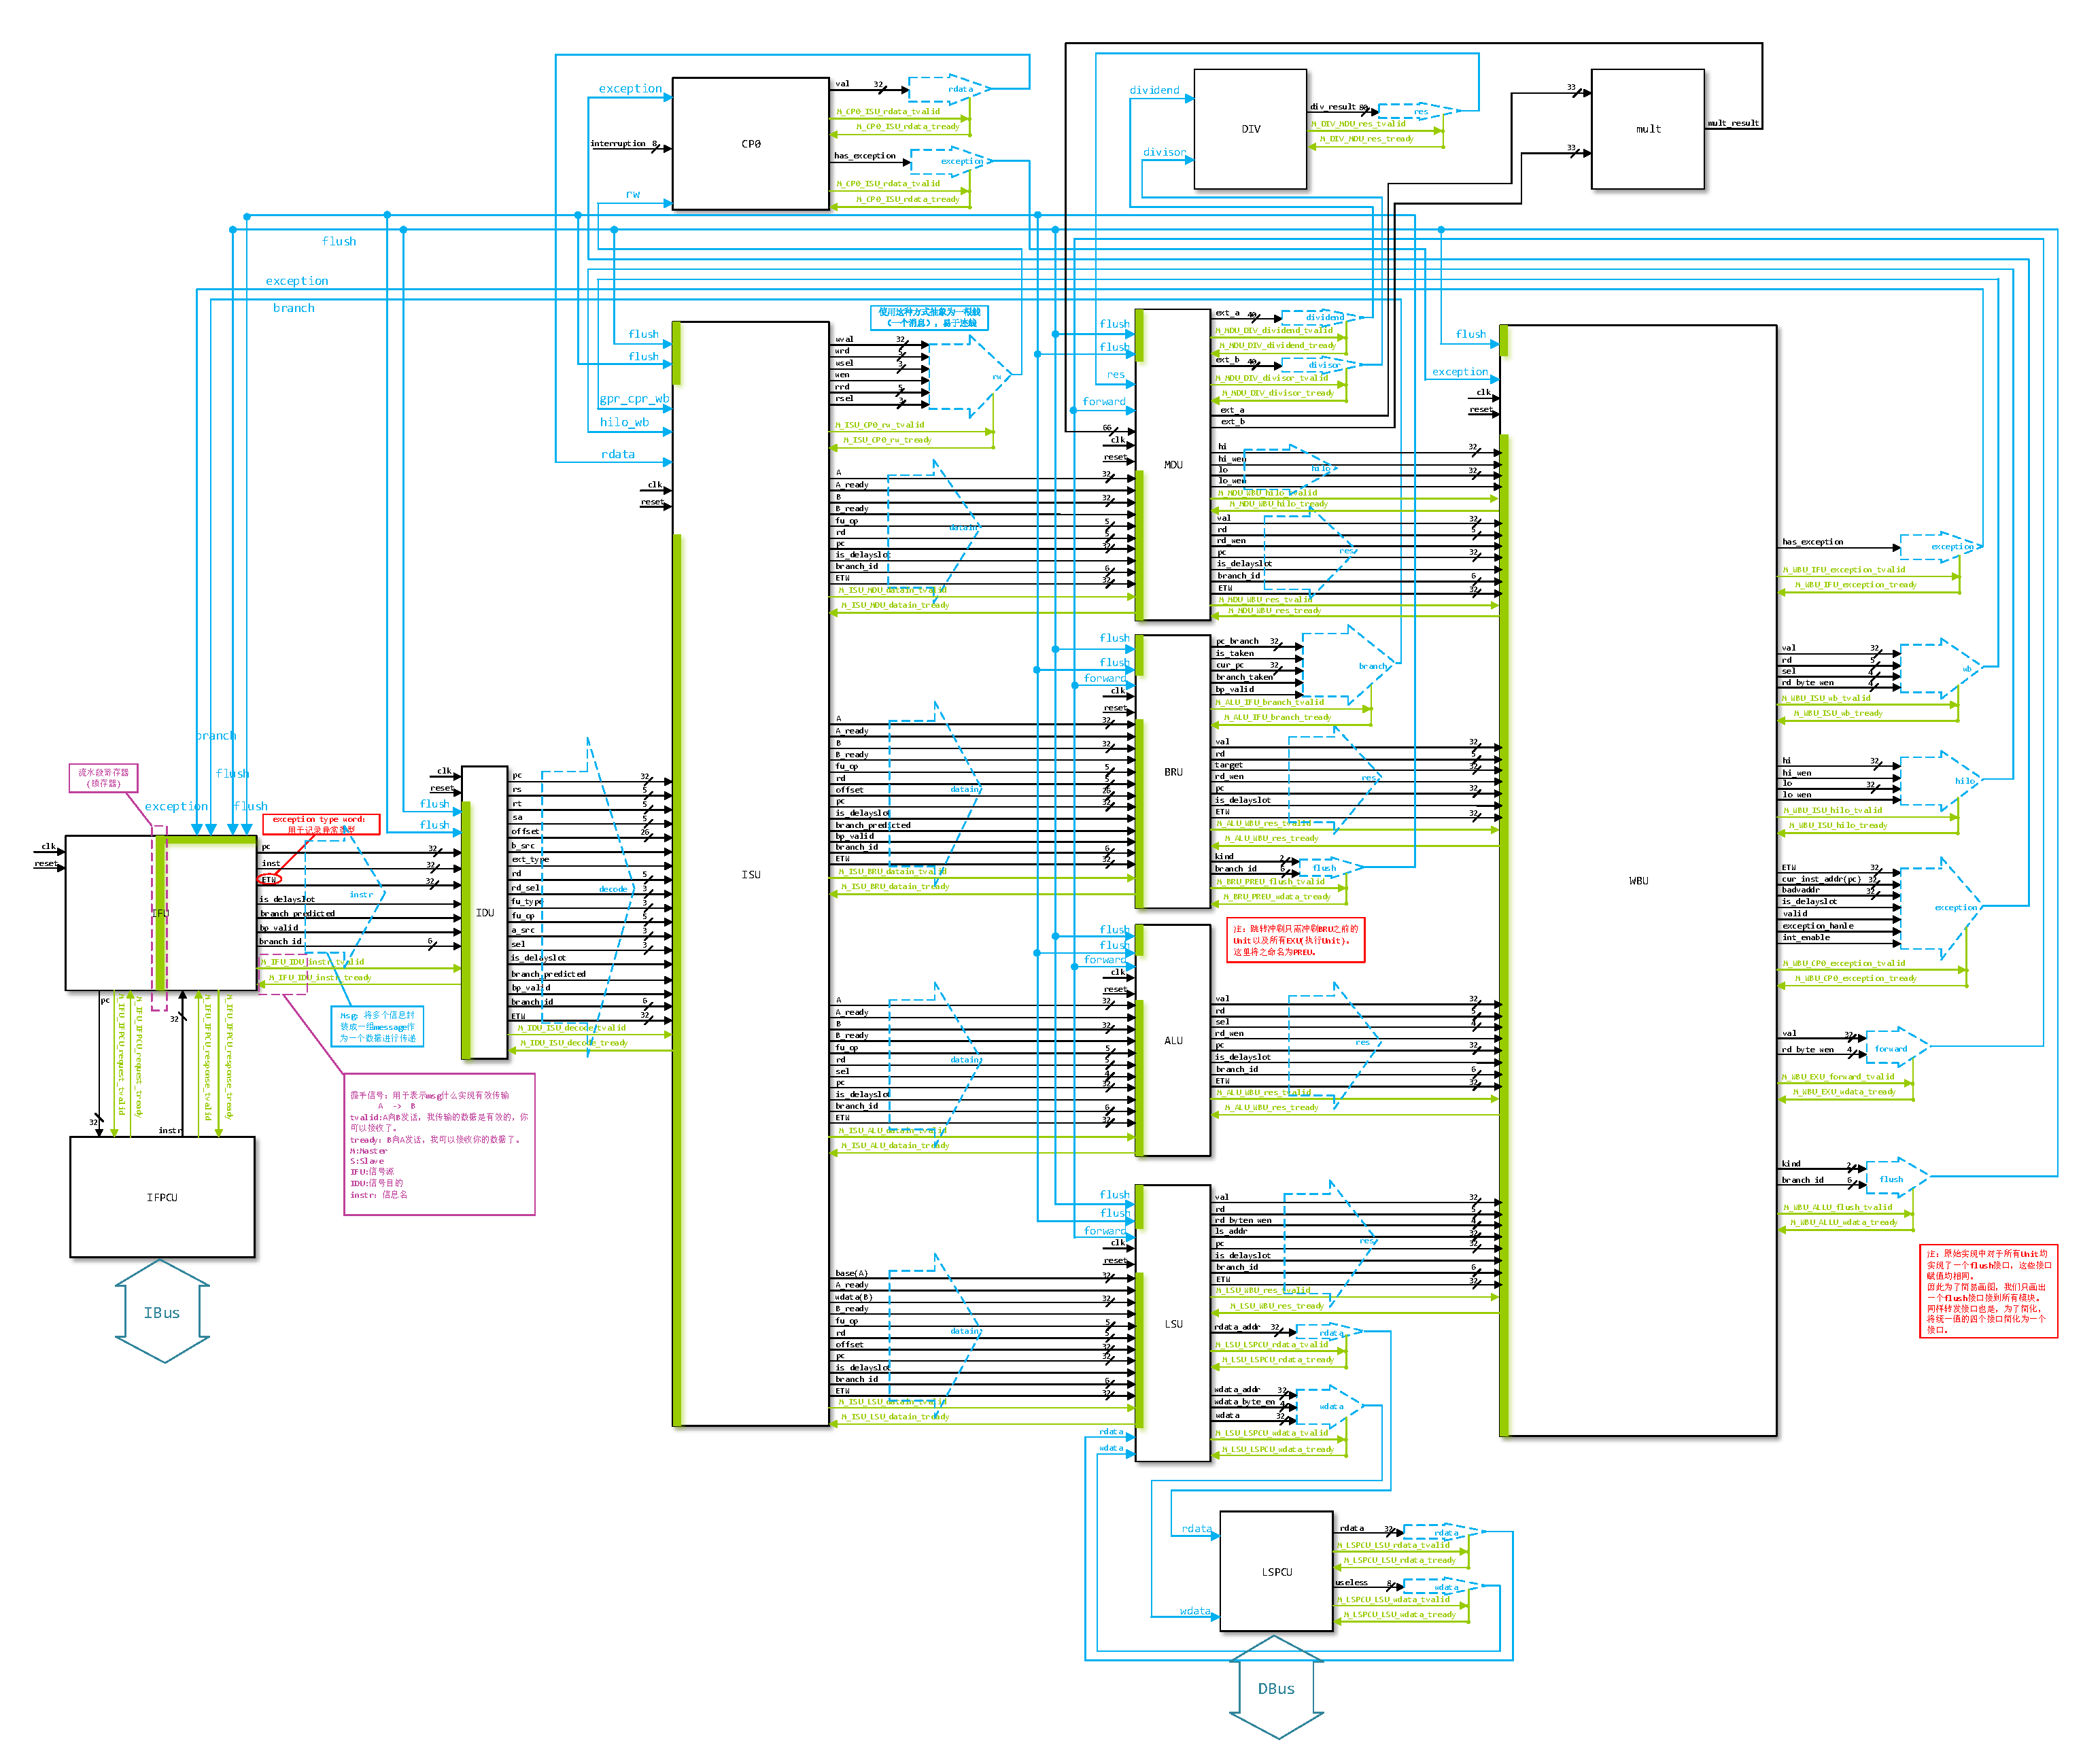
\includegraphics[width=\linewidth]{image/core-I4-2017}
\end{figure}

\section{往届core设计(2018)}

% \begin{tabular}{ll}
% Mass of empty crucible & \SI{7.28}{\gram}\\
% Mass of crucible and magnesium before heating & \SI{8.59}{\gram}\\
% Mass of crucible and magnesium oxide after heating & \SI{9.46}{\gram}\\
% Balance used & \#4\\
% Magnesium from sample bottle & \#1
% \end{tabular}
\subsection{模块设计图纸}

我们的cpu整体设计为6段流水线,如图\ref{fig:design_of_core}所示。由于初赛数据集较小,大部分数据集都可以直接装在l1 cache,l2 cache的设置在初赛中反而在某些数据集上起反效果,所以在最终提交的源码中,我们移除了这一组件。以及图中并未显式画出flush信号,这一信号用于分支跳转以及中断异常的冲刷。

\begin{figure}[htbp]
	\centering
	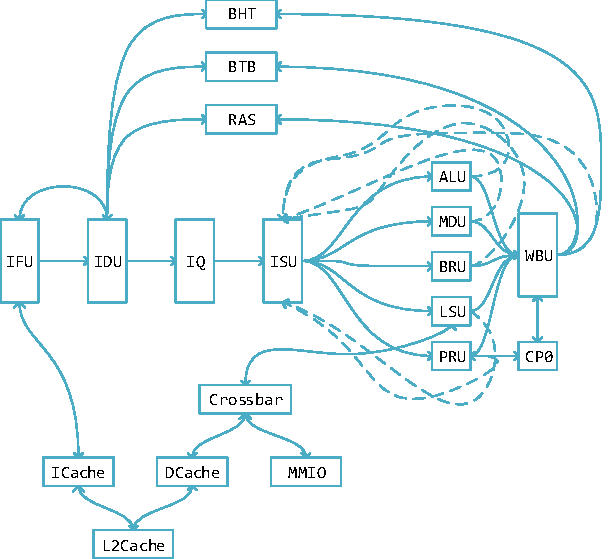
\includegraphics[]{image/core}\\
	\caption{CPU的核内设计}\label{fig:design_of_core}
\end{figure}

图中所有的执行单元和写回单元(wbu)均有一条虚线连接到ISU,这条虚线的含义是bypass信号,由于实际数据写回至少会晚上3个周期,为了能够更快的获取到寄存器数据,防止ISU因为等待数据就绪而空耗时间,项目添加了如图中虚线所示的bypass信号。

除了core,为了能够对接到龙芯的开发板,我们加入block design用于处理外围引线,其中block design的设计如图\ref{fig:design_of_uncore}所示:

\begin{figure}[ht]
	\centering
	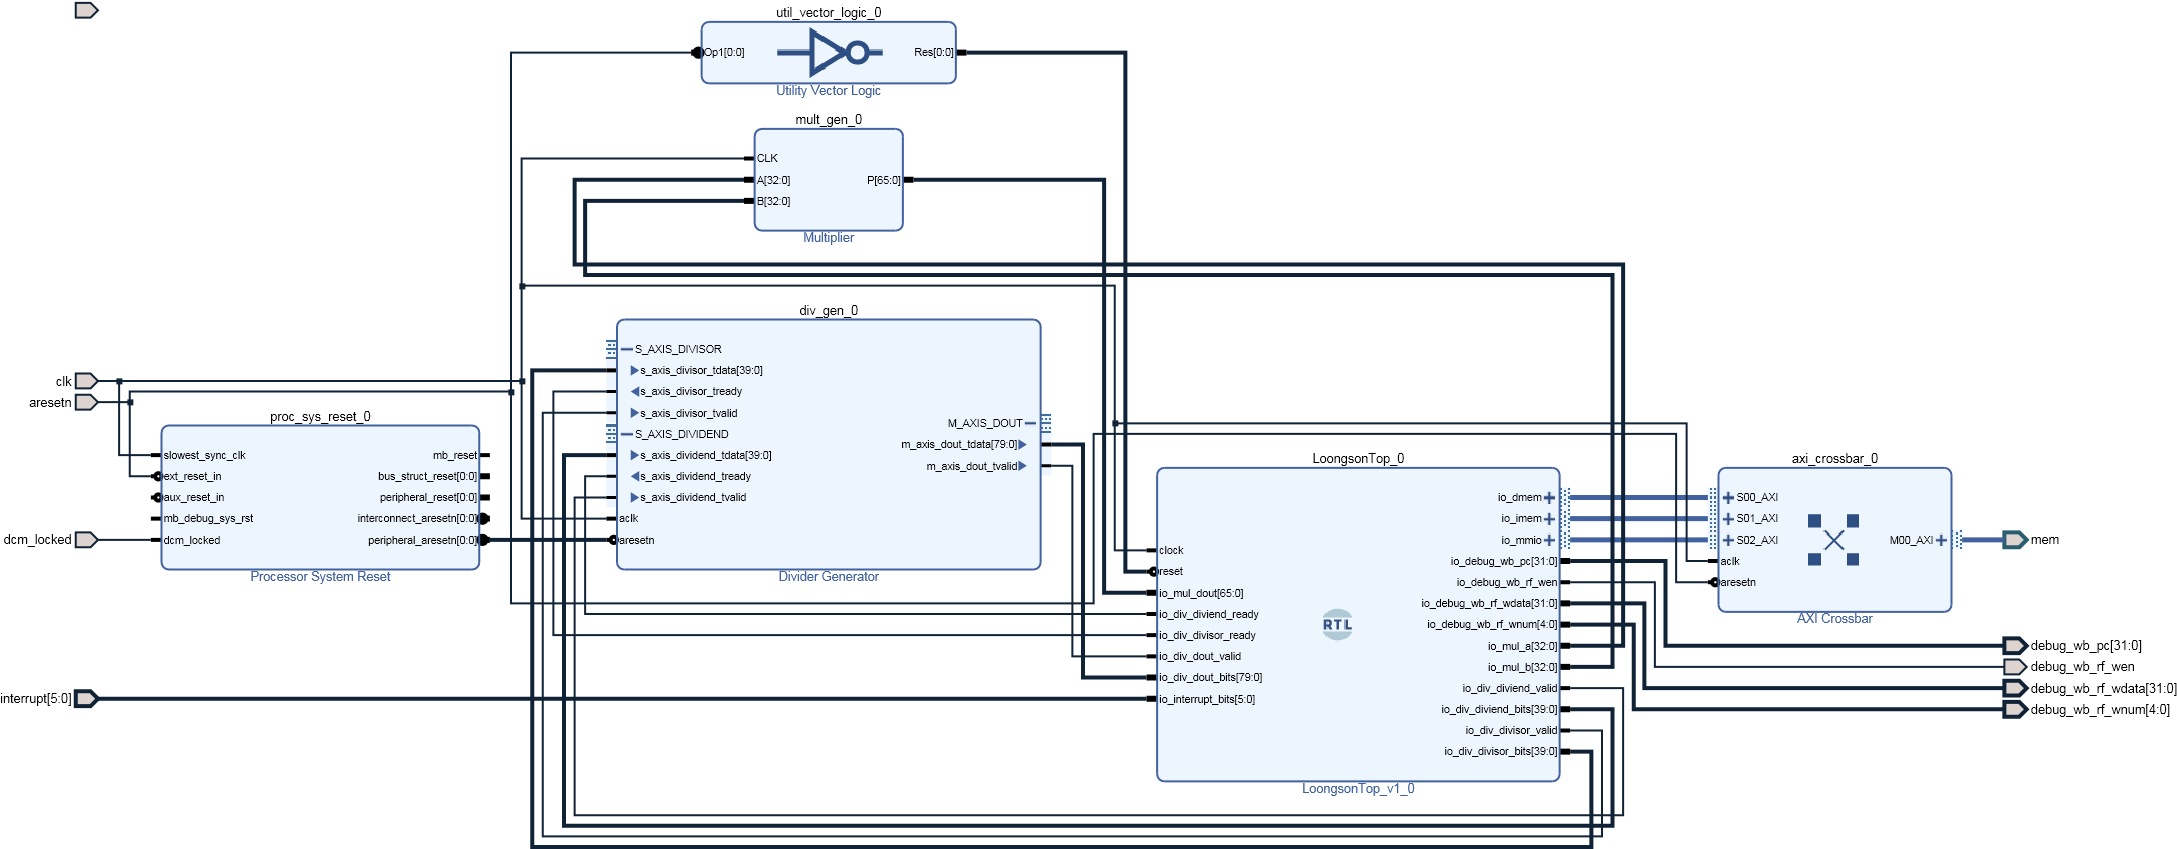
\includegraphics[width=\textwidth]{image/uncore.png}
	\caption{CPU的核外布线}\label{fig:design_of_uncore}
\end{figure}

\subsection{core模块简介}

CPU核心的架构如下图所示:

首先是IFU,取指单元。负责从icache中将指令取上来。由于icache存储使用的是block ram,而block ram是在下一周期返回读结果的,所以相应的,IFU是两级流水。第一级流水将PC发给icache,第二个周期从icache中将数据取上来。

接下来是IDU,译码模块。由于我们实现的是初步的乱序结构,在译码阶段,除了要完成指令的译码外,还要完成乱序需要的功能:
寄存器重命名:
对于源寄存器,要读取scoreboard,读取rename table
对于目的寄存器需要分配物理寄存器(处理WAW)
分配ROB
分配Branch ID
分配Load Store queue项,

分支预测:
分支预测模块包含了三样东西:
BHT,branch history table,负责进行分支预测,我们实现的是类似gshare的分支预测器。
BTB,branch target table,负责预测间接跳转指令的跳转地址。
RAS,RAS负责预测函数返回的跳转地址。

计分板
scoreboard中主要有:
32项的status,记录每个寄存器现在的状态。寄存器共有三种状态,他们的含义分别是:
SB\_READY:就绪态,这个寄存器的最新结果就在寄存器中。
SB\_BUSY:寄存器已经被重命名到ROB了,但是结果尚未就绪。
SB\_ROB\_READY:此寄存器已经被重命名到ROB中了,结果就绪,但是此指令尚未retire,所以结果要从ROB中读取。

ISU
然后是ISU,即指令发射队列,译码后的指令进入发射队列中,当源操作就绪,并且后端执行单元空闲时,即可读取发射操作数,并发射到后端执行单元执行。


后端执行单元:
后端执行单元执行完指令后,将指令状态以及计算结果写入ROB中,并通过bypass network传递到ISU。

ALU:计算算术逻辑指令
MDU:计算乘除法指令
PRU:处理cp0指令
BRU: 处理分支跳转指令

LSU: 处理load store指令
LSU以及Load Store queue的设计
LSU主要的工作是:
进行译码,地址生成,以及地址转换(查TLB),将指令派发到Load Queue以及Store queue。如果这条指令是load,则派发到Load queue,如果是Store,则派发到store queue。load queue、store queue的释放都是在指令retire后进行的。

ROB
reorder buffer,存储指令计算的结果,以及指令的例如pc、异常等基本信息。ROB是一条有序队列,每个执行单元到ROB都有一个写口,另外ROB有两个读口,用于ISU从中读取数据,另外ROB还有一个commit口。

WBU
当ROB头部的指令就绪时,它就可以commit了。然后它就进入了WBU,写回单元。写回单元检查指令是否出了异常,并进行相应的处理。另外,对于non-speculative load/store,WBU将他们对应的项从Load store queue中唤醒,并执行。

TLB
我们实现了64项TLB,支持虚拟内存。TLB本质上是一个大的CAM查找表。

L1 ICache、DCache
L1 ICache负责处理来自IFU的请求,DCache处理来自load store queue的请求,L1 ICache与DCache均用block ram实现,均为两级流水,在cache hit时,能一直流水。在cache miss时,则阻塞。另外L1 DCache支持背靠背的load,store,连续的load、store,store、load之间的数据转发均可以处理。

L2 cache
我们实现了L2 cache,AXI4接口,blocking,一次只能只能处理一个请求。由于龙芯测试集working set很小,所以在性能测试中,我们没有使用这个L2 cache。

\subsection{实现细节}

\subsubsection{未重命名的指令以及寄存器}

此外由于我们现在暂时没有对cp0寄存器以及Hi,Lo寄存器进行重命名,为了保持依赖,同时为了实现简便。现在在IDU阶段,cp0指令以及乘除法指令或者对上述寄存器的所有操作,都必须要等rob空了才会接着执行。IDU负责识别这些指令,并对前端进行必要的阻塞。

\subsubsection{发射队列的实现}

然后是ISU,即指令发射队列,译码后的指令进入发射队列中,发射队列中的每一项在进来的时候,都会记住自己的源寄存器的状态(在IDU阶段从scoreboard中读取),以及被重名到了ROB的哪一项。如果指令的源操作数的状态是SB\_READY或者SB\_ROB\_READY,则可以被直接发射,并不需要等待依赖满足。但是如果某一个操作数的状态是SB\_BUSY,则这条指令需要待在Issue queue中,等待唤醒。

issue queue中的指令主要要满足的依赖有:
源操作数就绪,执行单元空闲。

\subsubsection{唤醒操作}
我们从后端的每一个执行单元,以及WBU写回单元,都拉出一组线到issue queue,包含要结果就绪的寄存器下标、rob项下标以及算出来的值。我们将寄存器以及rob地址,与issue queue中的每一项进行比对,判断该条指令是否有源操作数就绪。这构成了wake up操作。另外,传递过来的算出来的新值,构成了bypass network。

\subsubsection{发射}
源数据就绪的指令,即可被发射,由于受发射宽度的限制(现在为1),我们用priority encoder选择一条指令出来发射。
指令在发射时读取源操作数,源操作数来自于:寄存器,ROB或者bypass network。
Speculative load、store。
由于对mmio的load/store以及对memory的store是有副作用的,为了实现精确内存,这些load store是必须在指令retire时才能执行的。而对memory的load,是可以推测执行的。


\subsubsection{精确内存,speculative load store}
由于mmio load/store,memory store是有副作用的,仅memory load无副作用。所以load queue中对memory的load是可以推测执行的,而对load queue中对mmio的访问,以及store queue中的任务是在指令retire后执行的。


\subsubsection{dynamic memory disambiguation以及维护memory RAW dependency}
由于指令是乱序发射并且load是允许推测执行的,所以可能出现新的load在老的store之前被issue到lsq,被执行完成,造成依赖关系错误。由于我们将load queue以及store queue实现成了两条无序queue,无法单从queue的位置关系,判断load,store指令间的先后关系。
同时,我们也没有实现store queue到load queue之间的bypass。
所以我们是在store指令retire时,将其地址与load queue中的每一项进行匹配,如果有匹配上的,并且已经执行的load,则说明出现了dependency failure,然后通过冲刷流水线来解决。这样子做是可行的,因为store指令是在retire时执行,此时,我们可以保证load queue和store queue中的指令都比它年轻。

\subsubsection{ICache、DCache一致性}
我们实现了Cache指令,支持ICache、DCache一致性。

\subsection{乱序处理器}
\subsubsection{从I4到IO2I}
我们在初赛时提交的版本是一个全顺序的流水线,In order fetch,in order issue, in order execute, in order retire,简称I4。
在初赛后,我们对其进行了下面这些提升,将性能测试跑分提升到了52分:
\begin{enumerate}

\item 更低的乘除法器延迟
\item 原有的实现中的cache line的valid,dirty均是用触发器实现,因为无法综合成BRAM,占据了大量的资源,影响了频率。在解决这个问题后,频率从70M提升到90M。
\item 提升分支预测准确率:
\begin{enumerate}
	\item perf test中的绝大部分测试需要很短的history,小部分,如bubble sort、quick sort需要很长的history,因此我们使用了两个history长度不同的BHT,并取预测效果最好的作为分支预测结果。
	
	\item RAS speculative update。由于流水线较长(主要是由于中间instruction
	queue的存在),而我们原来RAS压栈出栈都是在WBU阶段进行的,导致对于非常小的函数调用,call尚未commit,并将返回地址压入RAS,return就已经进了流水线了。我们支持了让RAS支持speculative update,在IDU阶段遇到call,return,就更新RAS。由于是speculative update,所以当出现分支预测错误时,RAS会进行部分恢复(恢复stack top指针)。添加了这个后,对于小函数调用多的stringsearch,提升明显,几乎所有的test的return预测错误,都降到了接近0%。
\end{enumerate}

\item DCache store、load bypass。对于stringsearch、stream copy等测试,存在明显的store,load背靠背的情况,我们处理了背靠背地址冲突的情况,加上了bypass。明显提升了这些项的分数。
\end{enumerate}


\subsubsection{IO2I:初步的乱序处理器}
in order fetch,OoO issue,OoO execute,In order retire。
此款处理器能够运行在70M,跑分33分左右。

考虑到乱序的复杂性,为了保证正确性,尽早拿出一个能够运行的版本,我们在实现中做了如下取舍,这保证了实现的低复杂度与正确定,但是性能不太好,甚至不如I4版本处理器。


1、显式重命名(重命名到物理寄存器)VS 隐式重命名(重命名到ROB)
重命名主要要处理好:

scoreboard:寄存器ready,busy状态
物理寄存器资源分配

对于scoreboard,这两种方案复杂性差不多。
但是对于物理寄存器资源的分配,差别则很大。
显式重命名需要实现active list,free list来维护物理寄存器的分配,在遇到分支时,需要做active list以及rename table进行check point,分支预测错误时需要进行回滚,复杂度更高。同时在异常时,需要walk back rob,复杂度太高。
上述这些可能看起来还不是太复杂,但是要考虑到:在checkpoint以及恢复free list,scoreboard以及rename table时,这些资源的分配,回收在同时进行,corner case非常多,不容易写对。一不小心就容易出现:
1、资源泄露,程序卡死(free list没有回收好)
2、依赖处理错误,程序错误(scoreboard没有处理好)
3、资源被重分配,程序错误(rename talbe没有处理好)

而隐式重命名只需要维护ROB,flush直接flush rob即可,不需要复杂的checkpoint以及恢复操作。

2、分支预测错误冲刷流水线的时机问题:
由于ROB的存在,如果在retire时冲刷,会导致分支预测错代价太大了,分支预测错要尽早flush。按理说,对于重命名到ROB的实现,只要将branch后的指令全部从rob中刷掉就可以了,由于我们需要scoreboard来维护寄存器是否ready,所以scoreboard必须要做checkpoint,这就又是一个复杂的点。
另外,由于我们要支持延迟槽指令,即使branch是放到了retire时冲刷,我们也不能直接对scoreboard进行reset,因为此时延迟槽指令还在流水线中。所以对于这种方案,我们也要对scoreboard进行checkpoint,并在flush时恢复。
为了让实现简单正确,我们采取的是分支预测错的flush,要等到延迟槽指令retire时,才发出,这样子可以保证流水线中没有任何处理器,scoreboard也可以直接flush,而不必进行checkpoint。

3、load store queue的实现
对于load store queue,由于我们采取的是load queue,store queue都是无序queue的实现,load指令无法判断哪条store比它老,因此也就无法进行数据bypass。我们采取了更加简单的方式来保证RAW dependency,store时,如果发现了有比它新的load被执行了,那就flush流水线。

4、简单实现的资源占用问题
对于单发射的乱序处理器,理论上,wake port可以只有一个,ROB的读口应该可以控制到三个(两个用来读数据,一个用来commit),写口应该限制到一个。
我们为了简单起见,所有的FU都是直接wake up issue queue,都直接将结果写入ROB,这导致了ROB的写口数量暴增,issue的CAM逻辑资源使用量也很大,进而限制了主频,以及issue queue与ROB的项数,进而限制了性能。

5、对Hi,Lo没有重命名,乘除法指令等待ROB空了再发射,这严重影响了coremark等乘除法密集型应用的性能。



如图\ref{fig:design_of_core}所示,图中列出了主要的core设计所涉及的模块,其中各个模块的含义大致描述如下:

\begin{enumerate}
\item IFU为取指单元,其通过握手信号向ICache发送取指信号,为了防止照成关键路径,ICache内部数据存储使用的是block ram,所以ICache在收到数据的下一周期才能返回数据,同时ICache的内部实现了流水化,所以迟一个周期返回数据几乎没有影响。

\item IDU为译码单元,用于对IFU取得的指令进行译码,以取得这条指令的操作数寻找模式,操作数扩展方式,访问的寄存器编号,写回的寄存器编号,所需发往的执行单元编号。

\item IQ为指令队列,用于存储所有已经译码成功的指令,为了防止后端执行周期过长阻塞前端。

\item ISU为分发单元,通过译码所得的结果读取寄存器,同时在寄存器读写约束不满足的时候进行必要的等待,索引转发结果。

\item ALU为算术运算单元,用于完成加法、减法、移位等可在一个周期内出结果的运算指令

\item MDU为乘除法单元,用于完成乘法和除法的运算,这一模块主体执行功能放在了核外的IP核上,而MDU内部逻辑主要是等待乘除法器的执行结果。

\item BRU为分支跳转单元,通过对ISU传入的操作数进行计算,以获取跳转目标,同时对于条件跳转指令还需要计算一下是否跳转

\item LSU为访存单元,用于load store指令的执行,若dcache miss,还需要额外的周期等待访存结果

\item PRU为特权指令单元,非特权指令不允许发送到这个单元,需要发送到这个单元的指令有MFC0、MTC0、SYSCALL、ERET,同时对于取指异常的指令和译码异常的指令,也需要发送到这个单元用以下拉异常信号

\item CP0为0号协处理器,用于完成中断异常主要计算功能

\item WBU为写回单元,用于将执行单元获取到的操作数写回到目标寄存器

\item BHT、BTB、RAS为分支预测单元,由于延迟槽的存在,整体的分支预测请求由IDU发出,并用于重定位IFU,wbu在写回寄存器时,也需要将BRU的计算结果更新到分支预测单元
\end{enumerate}

\section{往届core设计(woop)}

\begin{figure}[htbp]
	\centering
	\includegraphics[]{image/woop}\\
	\caption{CPU的核内设计}\label{fig:design_of_woop_core}
\end{figure}

\newpage

%\nocite{*}
%\bibliographystyle{unsrt}
%\bibliography{reference}

\end{document}
